% =============================================================================
% HealthEcon — paper source.
% Compiled locally; the PDF is git-ignored (see ../.gitignore).
% Style exemplar: Johnson & Rehavi (2016, AEJ:Policy); voice model:
% HomeOfficePNAD intro. Avoid em-dashes and long winding sentences.
%
% SUBMISSION TARGET: Journal of Health Economics (Elsevier). Per the JHE guide
% for authors: editable single-column .tex; abstract <= 250 words; 1-7 keywords;
% title page with full affiliations + corresponding author; references may stay
% in a consistent author-year style at submission (journal style is applied at
% proof); declarations (CRediT, competing interests, funding, data availability,
% generative-AI use) appear as unnumbered sections before the references.
% Highlights live in latex/highlights.tex and are uploaded as a separate file.
% Appendices A (model) and B (data) stay in the manuscript because they are
% needed to navigate the paper; Appendices C-E are the online supplement.
% =============================================================================
\documentclass[12pt]{article}

\usepackage[margin=1in]{geometry}
\usepackage{booktabs}
\usepackage{float}
\usepackage{graphicx}
\usepackage{amsmath}
\usepackage[round]{natbib}
\usepackage{caption}
\captionsetup{font=small,labelfont=bf}
\usepackage{rotating}
\usepackage{placeins}   % \FloatBarrier keeps sidewaystables in numbering order
\usepackage{xcolor}
\definecolor{citegreen}{RGB}{0,120,60}    % house green, as in HomeOfficePNAD
\usepackage[colorlinks=true,citecolor=citegreen,urlcolor=citegreen,linkcolor=citegreen]{hyperref}
\usepackage{xr}                    % cross-reference the online Supplementary Appendix
\externaldocument[]{supplement}    % resolves \ref{tab:...}/\ref{fig:...} to their C./D. numbers
\newcommand{\satab}[1]{Supplementary Appendix Table~\ref{#1}}
\newcommand{\safig}[1]{Supplementary Appendix Figure~\ref{#1}}

% Figure notes: a separate paragraph just below the caption title, styled small
% with a "Notes:" lead-in, so the figure title (\caption) stays clean and short.
% Typeset in a full-width minipage, whose \@parboxrestore cancels the float's
% \centering: the note is therefore justified at \linewidth, identical to the
% table notes built by standardize_notes() in analysis/code/00_utils.R. Do not
% narrow it or re-add \centering -- that is what made figure and table notes
% look misaligned.
% Figure notes must match the table notes: the same justified block at the FULL
% width of the text column (NOTE_OPEN / NOTE_CLOSE in analysis/code/00_utils.R).
% This is the Monasterio form. Do not narrow it, do not wrap it in \centerline,
% and do not re-add \centering; see the note-style history in CLAUDE.md.
\newcommand{\fignotes}[1]{%
  \par\vspace{1pt}%
  \begin{minipage}{\linewidth}\footnotesize%
  \textit{Notes:} #1%
  \end{minipage}}

% Title page in the Elsevier/JHE format: superscript-letter affiliations with
% city and country, and an explicitly marked corresponding author.
\title{Born on Schedule: Fees, Supply-Side Scheduling, and Cesarean Delivery
in Brazil}
\author{Fredie Didier\textsuperscript{a,}\thanks{Corresponding author.
E-mail: fdidier@terra.com.br.}
\and Vinicius Mendes\textsuperscript{b}
\and Pablo Castro\textsuperscript{b}
\and Lucas Emanuel\textsuperscript{b}}
\date{}

\begin{document}
\maketitle

\vspace{-1.5em}
\begin{center}\small
\textsuperscript{a}\,Instituto Brasileiro de Ensino, Desenvolvimento e Pesquisa
(IDP), Bras\'ilia, DF, Brazil\\
\textsuperscript{b}\,Federal University of Bahia (UFBA), Salvador, BA, Brazil\\[2pt]
E-mail addresses: fdidier@terra.com.br (F. Didier), vdmendes@ufba.br
(V. Mendes), pablocastro@ufba.br (P. Castro), lucasemanuel@ufba.br (L. Emanuel).
\end{center}

\begin{abstract}
\noindent Brazil's for-profit hospitals deliver about 81 percent of their births by
cesarean, yet under private insurance a cesarean pays the physician less, on
average, than a vaginal delivery once the hourly labor-assistance fee is
counted. We combine the universe of private-insurance claims, which record the
physician fee of nearly every delivery, with 42 million birth records that flag
cesareans performed before labor. In the five largest states a cesarean pays 18
to 38 percent less, and the literature's fee responses imply at most 1.4
percentage points from a gap of this size. Per hour of physician time the
ranking reverses: a one-hour cesarean pays more, on average, than a vaginal
delivery lasting over about 1.25 hours. For-profit cesarean rates fall 7.9
percentage points on weekends and public ones 6.7, mostly among cesareans
performed before labor. In the same municipality and day, the for-profit decline
is 1.8 points larger on weekends and 2.5 on holidays, essentially unchanged when
maternal composition is held fixed. Within Robson clinical groups, practice
style accounts for 73 percent of the 36-point for-profit--public gap, and
for-profit births are 12.2 points more likely to be early-term after maternal
controls. Most of the calendar gradient is common to both sectors, which we read
as organizational; the for-profit increment is consistent with a price of
physician time that the fee schedule pays only for billed labor hours. The
evidence points to the organization of obstetric time, rather than the relative
procedure fee, as a promising policy margin.
\end{abstract}

\bigskip
\noindent \textbf{JEL classification:} I11; I13; J22; D82.

\begin{sloppypar}
\noindent \textbf{Keywords:} cesarean section; physician agency; supplier-induced
demand; supply-side scheduling; Brazil.
\end{sloppypar}

\newpage

% =============================================================================
\section{Introduction}\label{sec:intro}
% =============================================================================

Cesarean section is the most common major surgery in the world, and its use has
risen far beyond any clinical benchmark. About 21 percent of births worldwide are
cesarean deliveries, a share projected to reach nearly 29 percent by 2030
\citep{betran2021}. The World Health Organization sets no target rate. Its current
position is that population-level gains in maternal and newborn survival stop
appearing above a cesarean share of about 10 percent, and that institutions should be
compared through the Robson classification of deliveries rather than against a
headline number \citep{who2015cesarean}. We use that classification throughout.
Overuse is not innocuous: unnecessary
cesareans raise maternal morbidity, respiratory distress and other neonatal
complications, and costs \citep{sandall2018,boerma2018}. Brazil is the frontier
case: roughly 56 percent of all Brazilian births are cesarean. In the private-insurance
sector, which covers about a quarter of the population, the rate reaches about
84 percent, and at for-profit birth establishments in the registry it is about 81 percent.
Among the 85 countries in which more than 95 percent of births take place in a
health facility, only the Dominican Republic has a higher national cesarean rate
than Brazil \citep{boerma2018}. The excess is
not confined to complicated pregnancies. Among first-time mothers at term with a
single, well-positioned baby who are already in spontaneous labor, the group for
which surgery is hardest to justify on clinical grounds, 68 percent of for-profit
weekday deliveries end in a cesarean, against 36 percent in public
hospitals. Understanding what sustains surgical rates of this magnitude in a
modern, well-financed health sector is a first-order question for health policy
well beyond Brazil.

When patients cannot judge treatment necessity, physicians act as imperfect
agents and can tilt clinical decisions toward their own interests
\citep{dranove1988,mcguire2000}. The canonical version of this argument is
financial: providers do more of what pays more. \citet{gruber1996physician} show
that obstetricians perform more cesareans when a falling birth rate squeezes
their incomes, \citet{gruber1999physician} estimate the response of the cesarean
rate to the cesarean--vaginal fee differential across Medicaid programs, and
\citet{clemens2014} document strong treatment responses to payment changes in
Medicare. The financial channel is not universal, however. In childbirth,
\citet{grant2009} re-estimates that fee response on corrected data and finds it
about a quarter as large as originally reported, and \citet{alexander2020} finds
that bonuses paid to physicians for cutting the hospital costs of Medicare
patients changed which patients they admitted but not, given patient health, the
procedures they used. The sharpest counterexample
comes from Chile. \citet{elejalde2021} study a reform that moved publicly insured women into
private hospitals paid the same price for a vaginal delivery and for a cesarean,
and find the cesarean rate rose by 8.6 percentage points anyway. They attribute
the increase to schedulability: a cesarean can be booked, which lets a hospital
move deliveries off weeks it expects to be crowded and take more deliveries in
total. Removing the price differential did not remove the incentive to operate.
Childbirth has become the
laboratory of choice for testing physician agency, precisely because the cesarean
decision is frequent, discretionary, and well measured: \citet{currie2008} show
that
liability pressure distorts delivery mode, \citet{johnson2016} find that
physicians treat informed patients (other physicians) differently from everyone
else, and \citet{card2023} find that among low-risk first births a hospital's
cesarean propensity has offsetting effects on the newborn, improving condition at
birth by averting prolonged labor while raising later respiratory presentations. Throughout most of this literature the
operative margin is money. Yet the physician's scarcest input is not billable
revenue but time. A vaginal delivery is a long commitment of uncertain onset and
duration that blocks nights, weekends, and office hours; a scheduled cesarean is
a one-hour appointment at a time of the physician's choosing. Separating the
price of the procedure from the price of the physician's time requires observing
actual physician fees and the exact timing of births in the same setting, a combination
administrative data rarely provide.

That births in Brazil follow the calendar is itself documented:
\citet{spinola2026} find birth-timing manipulation around public holidays and
medical congresses, markedly stronger in the private sector, and \citet{melo2024}
estimate birth displacement around Carnival. Our contribution is not the weekly
birth cycle but a joint diagnosis. We observe the two central inputs of the
physician's choice in the same national setting, the fee actually billed and the
timing of delivery, and we compare for-profit with public establishments within
the same municipality and day. The relative procedure fee cannot carry the
epidemic, but per hour of physician time the cesarean is the better-paid
procedure. Three calendar fingerprints, the weekend and holiday declines, the
business-hour concentration, and the prelabor-versus-in-labor split, point to
supply-side scheduling in both ownership sectors. The for-profit--public
comparison and the Robson decomposition then isolate the part specific to
for-profit establishments, the one a price of physician time can speak to.

This paper separates the two channels at national scale, combining two
administrative universes. The first is the set of private-insurance hospital
claims filed with the sector's federal regulator under Brazil's mandatory
reporting standard (Troca de Informa\c{c}\~oes na Sa\'ude Suplementar, TISS),
which records the physician fee actually billed for 95.5 percent of deliveries
from 2015 to 2024. The second is the Ministry of Health's register of live births (Sistema de
Informa\c{c}\~oes sobre Nascidos Vivos, SINASC), 42 million births from 2010 to
2024 with the exact date and hour of birth, the clinical group under the World
Health Organization's Robson classification, and an indicator for whether a
cesarean was performed before labor began. The claims measure what a delivery pays,
per procedure and per billed hour; the birth records show when deliveries happen. The empirical strategy exploits
two sources of variation: differences in relative fees across municipalities and
over time to test the price channel, and the calendar distribution of observed
births, together with prelabor timing and within-municipality-day sector
comparisons, to characterize the scheduling channel. Three sets of facts
emerge.

First, the relative procedure fee cannot account for the epidemic, while the
price of the physician's time favors the cesarean. Per delivery, the correct comparison credits
the vaginal delivery with the separately billed hourly labor-assistance fee,
billed with 38 percent of vaginal deliveries for 2.9 hours on average at roughly
R\$420 per hour. Once it is counted, a cesarean pays the physician 18 to 38 percent less
than the average vaginal delivery in Brazil's largest states, which nonetheless run cesarean
rates of 78 to 90 percent under private insurance. Per hour of physician time the ranking reverses: a cesarean pays
about R\$1,940 for roughly an hour of surgery booked in advance, so it pays more
per hour than the average vaginal delivery once that delivery occupies the physician for
longer than about 1.25 hours, and the labor hours that are billed already average 2.9. The
fee responses the literature has established show how little the relative fee can
do: at the response \citet{gruber1999physician} estimate, the negative fee gap of
Brazil's largest states moves the cesarean rate by at most about 1.4 percentage
points, and by at most about a third of a point at the smaller response
\citet{grant2009} obtains on corrected data, against a for-profit--public gap of
36 points. Our own fee regressions, across municipalities and years and with
controls for local income, insurance coverage, prenatal care, and obstetrician
supply, disagree with one another and do not settle the magnitude: the
within-municipality intervals exclude both of the literature's responses from
below, while the state-level estimate without controls lies above the larger one.
Even that largest estimate, applied to the fee gap of the largest states, would
move the cesarean rate by about 2.4 percentage points.

Second, the calendar carries a pattern that the fee data do not. The natural
onset of spontaneous labor ignores the week, but the observed delivery date can
be moved through induction and prelabor scheduling, so systematic weekly patterns
in surgery document how deliveries are ordered across dates. That delivery dates
are shifted for non-clinical reasons is well established: births respond to tax
and transfer incentives \citep{dickertconlin1999,gans2009}. Our central estimate compares for-profit with
public establishments within the same municipality and the same day, so
that municipality-by-date fixed effects absorb every shock the two sectors share
on a given local day. That comparison leaves a for-profit-specific weekend decline
of 1.8 percentage points and a holiday decline of 2.5 points, essentially unchanged
at 1.8 and 2.4 once the predetermined maternal composition of each cell is held
fixed. Half or more of the weekend differential is a change of practice within the
same establishment, and the rest is weekend births moving toward establishments
that deliver fewer of them by cesarean. Each sector's own gradient is much larger. Cesarean rates at for-profit
establishments fall by 7.9 percentage points on weekends and 5.3 points on
national holidays, against 6.7 and 3.5 points at public ones, and half of all
cesareans are performed in weekday business hours, against a 30 percent benchmark under
uniform timing. Weekly scheduling therefore pervades Brazilian obstetrics and
most of the gradient is common to both sectors; what distinguishes the for-profit
model is the differential on top of it.
The mechanism is visible in the components of the rate: at
for-profit establishments the weekend dip is minus 8.9 percentage points for
cesareans scheduled before labor and slightly positive, at 1.9 points, for
cesareans during labor, so it is concentrated in surgery booked in advance. It
does not vanish among low-risk first-time mothers already in spontaneous labor;
most of that dip is among cesareans coded as performed during labor, a part that
reflects intrapartum decisions and selection rather than prelabor scheduling.
The same pattern appears across the clinical
classification: the excess for-profit weekend gradient is concentrated in the
term, singleton, cephalic pregnancies without a previous cesarean, where the
choice between labor and surgery is most open. It disappears among preterm
births, whose delivery date is less often chosen in advance, and it reverses
where surgery is already close to universal, as among women with a previous
cesarean, whom for-profit establishments deliver by cesarean 95 percent of the
time on weekdays. Two extensions come back weaker than the
mechanism predicts. Holidays that create a long weekend do not produce larger
dips than genuinely isolated Wednesday
holidays, and there is no bunching of prelabor cesareans in the days before a
long block; instead, for-profit obstetric activity is depressed across the entire
holiday period. And within for-profit establishments the calendar gradient is flatter at larger
obstetric services, and the data do not apportion that attenuation between bed
count and delivery volume. Entered together with date fixed effects, only volume
is significant; under municipality-by-date fixed effects, which remove much of
the variation that identifies both, the two are jointly significant but neither
is distinguishable from zero on its own. The evidence therefore documents a supply-side calendar
pattern consistent with scheduling, common to both ownership sectors and stronger in
the for-profit one, without identifying the causal effect of scheduling or whose
constraints generate it.

Third, the for-profit practice style has a size and a cost. A decomposition over Robson
clinical groups attributes 73 percent of the 36 percentage-point for-profit--public gap to
practice style within the same clinical groups, not to differences in case-mix.
Benchmarking each municipality's weekday cesarean propensity against its own
weekend rate places about 35,000 for-profit weekday cesareans per year above that
mechanical benchmark, about one in eleven of the cesareans the sector performs on
weekdays, a count of surgery
above the weekend rate rather than of procedures that scheduling alone caused. The
for-profit sector also delivers earlier: for-profit births are 12.2 percentage points more likely to occur
at 37--38 weeks of gestation than public births after controlling for maternal
age, education, and race, and prelabor cesareans are the earliest of the three
delivery types.
Early-term delivery is the margin that the clinical literature links
to higher neonatal respiratory morbidity and intensive-care admission
\citep{tita2009}, and quasi-experimental evidence links non-indicated
cesareans and earlier scheduled births to worse newborn health
\citep{costaramon2018,borra2019}.

The calendar regressions identify the ordering of deliveries across dates, not the
total number of cesareans caused by scheduling. Equation~\eqref{eq:gradient}
provides a within-municipality-day for-profit--public differential under a
common-gradient assumption, while the gestational-age results remain
associational. Section~\ref{sec:strategy} states these estimands and assumptions
formally.

A simple model of physician time rationalizes these facts. A physician weighs the
fee gap against a convenience premium, the value of converting an unschedulable,
calendar-blocking delivery into a one-hour appointment. The premium is the price
of the on-call and unbilled time that the fee schedule omits, and because it is
positive, a cesarean can be chosen even where the per-delivery fee gap is
negative, as it is in the largest states. The model does not by itself imply
that the relative procedure fee has little traction; that conclusion rests on
the calibration, which places the fee responses documented in the literature far
below the size of the gap.

The paper contributes to three literatures. The first is the
economics of
physician agency and supplier-induced demand \citep{mcguire2000,%
gruber1996physician,gruber1999physician,clemens2014}. That literature has
established that providers respond to financial incentives, and the canonical
test is whether treatment intensity tracks fees. We bring a setting where billed
fee differences can be measured directly. Across the observed variation, the
estimates do not provide stable positive support for the financial channel:
cesarean use does not track the fee gap, and it is high precisely
where cesareans pay less per procedure. In its place we document not a non-price
margin but a price the fee schedule sets only in part, the price of the
physician's time: billed labor hours are paid, while on-call availability and
unbilled hours are not. We also document the behavior it predicts: supply-side scheduling of surgery around the
calendar, which the model attributes to the opportunity cost of physician time. Our data locate the margin
on the supply side but cannot separate the attending physician's own time from
hospital staffing, operating-room capacity, and scheduling protocols, so we frame
the mechanism as supply-side convenience scheduling rather than as a clean
measurement of the physician's private opportunity cost. This reframes
supplier-induced demand around the price of time, a margin the fee schedule
prices only in part. Brazil is the sharper version of the Chilean case in
\citet{elejalde2021}: the fee gap here is not merely absent but negative, and
cesarean use is high anyway. Their mechanism and ours are siblings, and they are
separable in these data, because theirs is seasonal, a hospital levelling its
throughput across weeks, while ours is weekly, present in both ownership sectors
and stronger in for-profit ones. We test theirs directly and do not find it. Prelabor timing does not
respond to the demand an establishment can forecast for the following week, a
test that bounds only large responses because the forecast is weak, and the
sharper implication finds no levelling: establishments that schedule more show no
smoother weekly delivery flow (\satab{tab:demand_smoothing}). The paper also connects to the literature on
physician practice styles and geographic variation in treatment, which finds
that much of the variation in care reflects supply-side practice patterns rather
than patient case-mix \citep{finkelstein2016,molitor2018,cutler2019,%
curriemacleod2016,fischer2026}. We show that in one of the most extreme cesarean
systems on record practice style within the same clinical groups accounts for
most of the for-profit--public gap, and that this practice follows the working
week. Recent work shows that maternity-ward capacity and
workload alter obstetric procedure use: \citet{maibom2021} and \citet{bensnes2026}
exploit day-to-day maternity-ward crowding, \citet{facchini2022} studies cesarean
use under low midwife staffing, and \citet{bachner2024} find that empty
maternity beds raise the probability of a cesarean. In Brazil, \citet{parfitt2026} show that
heat stress changes the allocation of deliveries between physicians and nurses
and, conditional on physician attendance, increases prelabor cesareans. This
literature motivates our broader organizational interpretation: the calendar
gradient may reflect staffing, capacity, and scheduling protocols as well as the
attending physician's private convenience.

The second is the economics of childbirth, where the cesarean decision has
become a workhorse for studying physician behavior \citep{currie2008,%
johnson2016,costaramon2018,card2023}. \citet{johnson2016} use information
asymmetry between doctor and patient, and \citet{currie2008} use liability
pressure, to move the delivery-mode margin; \citet{epstein2009} document
persistent physician-specific treatment styles in cesarean use, and
\citet{card2023} trace the consequences of delivery practices for newborn health.
Our contribution is a national empirical anatomy of this system, assembled from the
universe of private-insurance claims and birth records, with mechanism evidence
on the timing of surgery and a within-municipality-day differential between
for-profit and public establishments. Our calendar evidence relates most directly to work connecting
provider incentives and convenience to the timing of delivery
\citep{cohen1983,brown1996,spetz2001,fabbri2016,jacobson2021}, and within Brazil
to the holiday and Carnival evidence of \citet{spinola2026} and \citet{melo2024}.
Relative to this literature, we combine actual billed physician fees,
same-municipality-day ownership contrasts, prelabor timing, Robson-group
composition, and establishment capacity. The closest contemporaneous study is
\citet{parfitt2026}, who exploit short-run temperature variation in Brazilian
public maternity wards to estimate equilibrium changes in provider attendance
and delivery practices. Our question and estimand differ: we study a persistent
weekly calendar gradient, common to both ownership sectors and stronger in the
for-profit one, and our municipality-by-date fixed effects
absorb temperature and every other local daily shock common to the two ownership
sectors. The paper therefore adds evidence on the relationship between payment,
ownership, and the organization of obstetric time, not another estimate of the
effect of environmental stress.\footnote{Sector definitions are not directly comparable across
studies. \citet{parfitt2026} analyze deliveries in public maternity wards;
\citet{melo2024} classify hospitals using the allocation of obstetric beds
across public and private care; our SINASC comparison uses the establishment's
legal ownership status. We therefore compare mechanisms and calendar responses
across papers, not coefficients for identical institutional populations.}

Brazilian studies of birth-timing manipulation motivate scheduled cesareans by
combining compensation and time incentives \citep[e.g.,][]{melo2024}: the
procedure is believed to pay more, to require less provider time, and to be
schedulable more predictably. Our claims data separate these components: once separately
compensated labor assistance is included, the payment premise is not generally
supported per procedure over the observed fee variation, whereas the business-hour, weekend,
holiday, and prelabor patterns point to a time-and-organization margin.
Families may also manipulate birth dates in response to financial incentives or
culturally salient dates \citep{dickertconlin1999,gans2009,gans2012,lo2003}. Our
stronger prelabor gradient in for-profit establishments is more consistent with
a supply-side organizational margin, but it does not exclude joint
physician--patient scheduling.

The third is the design of health policy in middle-income countries. Brazil aimed
the fee schedule, mandatory disclosure, and a quality program at the epidemic over
a decade. The national package lowered the cesarean rate by an estimated 1.6
percentage points \citep{melo2023}, and the for-profit rate was still about 78
percent in 2024. The two leading episodes motivate, but do not identify, the
effect of alternative policies: the court order never changed relative fees,
and the observational evaluation of the flagship quality program, Parto Adequado
(``Adequate Childbirth''), cannot separate the program from a downward trend at
participating hospitals that began well before they joined (Supplementary
Appendix Figures~\ref{fig:pa_hospital} and~\ref{fig:rn368}). The evidence
redirects attention from relative fees to the organization of obstetric time,
the on-call coverage and scheduling norms that determine the convenience
premium, as the margin worth testing.

The remainder of the paper proceeds as follows. Section~\ref{sec:background}
describes the private health sector, delivery payment, and the policy
environment. Section~\ref{sec:data} presents the two administrative datasets and
the construction of the analysis files. Section~\ref{sec:strategy} lays out the
estimating equations and the identification logic behind each of them.
Section~\ref{sec:notprice} compares the fees per procedure and per hour of
physician time and calibrates the response to the relative fee.
Section~\ref{sec:mechanism} presents the scheduling evidence and its checks. Section~\ref{sec:cost} quantifies the
epidemic's composition and its gestational-age margin, and
Section~\ref{sec:conclusion} concludes. Appendix~\ref{sec:model} develops the
model.

% =============================================================================
\section{Institutional background}\label{sec:background}
% =============================================================================

About a quarter of Brazilians hold private health
insurance,\footnote{See \href{https://www.gov.br/ans/pt-br/acesso-a-informacao/perfil-do-setor/dados-gerais}{ANS (2026)}.}
a parallel system
of insurers and accredited hospitals regulated by the federal
private-health-insurance authority, the National Supplementary Health Agency
(Ag\^encia Nacional de Sa\'ude Suplementar, ANS). The rest rely on the public
single-payer system, the Unified Health System (Sistema \'Unico de Sa\'ude, SUS).
Childbirth is covered by both, but the two sectors deliver very differently.
Figure~\ref{fig:trend} plots the cesarean share of births by sector over time.
In the private-insurance claims the rate stays between 82 and 86 percent in every year,
and at for-profit birth establishments it is about 81 percent over the period; in the
public sector it rises from about 37 percent to about
52 percent. All three are far above the population share at which the World
Health Organization finds survival gains to stop.

\begin{figure}[H]\centering
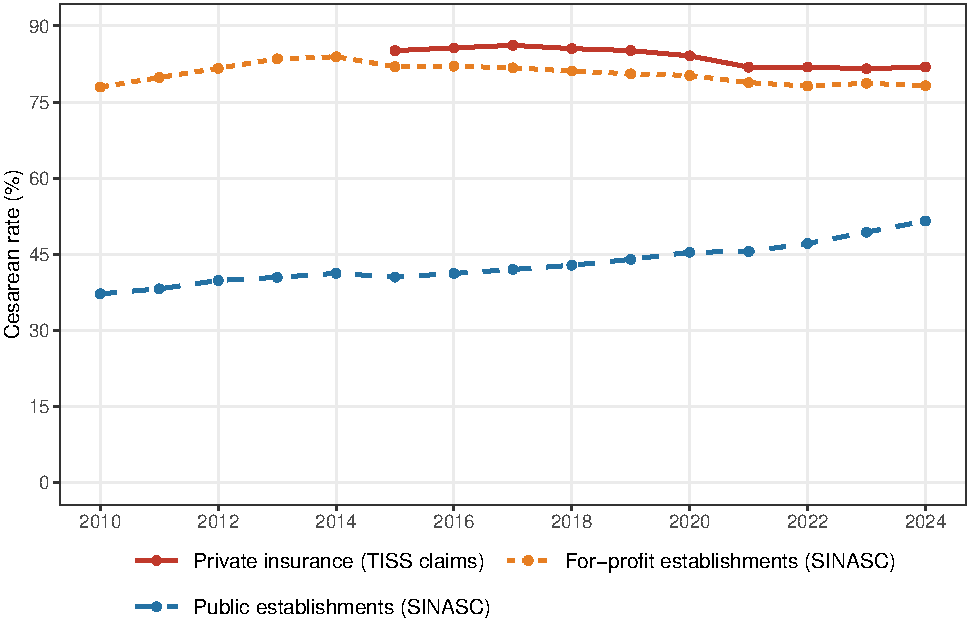
\includegraphics[width=\textwidth]{../analysis/output/graphs/fig01_csection_trend.pdf}
\caption{\textbf{Cesarean rate by sector, 2010--2024}}\label{fig:trend}
\fignotes{Cesarean share of deliveries. ``Private insurance (TISS claims)'' is the
insurance-financed sector; ``For-profit / Public establishments (SINASC)''
classify births by the legal-entity type of the birth establishment.}
\end{figure}

High cesarean rates cover the Center-South and much of the country rather than a
few states, with the lowest rates in parts of the North;
\safig{fig:map_private} maps the private-insurance cesarean rate by municipality.

In the private-insurance sector, obstetricians are paid fee-for-service on a procedure schedule. A
delivery generates a fee for the procedure itself, and a vaginal delivery
additionally generates a separately billed ``labor assistance'' fee for each
hour spent attending labor. This detail matters for measuring
incentives and is central to Section~\ref{sec:notprice}.

A second payment sits outside the claims. A beneficiary who wants the obstetrician
who followed her pregnancy to attend the delivery, whenever it happens, may be
asked for an ``availability'' fee. The Federal Council of Medicine holds that such
an agreement is ethical only if the patient then pays the delivery fee in full and
the plan pays nothing for it \citep{cfm2012disponibilidade}. The regulator calls
such charges improper \citep{ans_parto_direitos}, and its board has ruled that a plan whose beneficiary
refuses the fee must provide an obstetrician who does not charge it, failing
which it denies coverage \citep{ans2014disponibilidade}.
Where it is charged, the delivery reaches the claims without a physician delivery
fee, and the fee itself is a price for the obstetrician's time. Continuity of this
kind differs sharply between the two sectors. In a national hospital-based cohort of
2011--2012, about 77 percent of women whose delivery was privately paid were
delivered by the professional who had followed their pregnancy, against about 9
percent of those whose delivery was publicly paid, whose hospitals staff
deliveries with teams on duty \citep{domingues2014}.

Three policy episodes recur in the paper, and their institutional scope differs.
Resolution RN 368/2015 is a national ANS rule, binding on all
private plans, that created a right to operator-, hospital-, and
physician-specific cesarean rates on request and made the partogram and an
informed-consent term mandatory for elective cesareans. In December 2015 the
Federal Court in S\~ao Paulo, ruling on a civil action by the state prosecutor,
ordered the ANS, a national regulator, to issue rules making plans pay at least
three times more for vaginal than for cesarean delivery; the agency appealed, and
the rule never took effect. Parto Adequado (``Adequate Childbirth'') is a
national quality-improvement program run by the ANS together with a large private
hospital and the United States-based Institute for Healthcare Improvement;
adoption is voluntary and at the hospital level, with a 2015--16 pilot and a
2017--2021 dissemination phase of about 113 hospitals in 60 municipalities.
\citet{melo2023} evaluate the national policy package of this period, whose
supply-side component restricts elective cesareans before 39 completed weeks, and
estimate a reduction of 1.6 percentage points in the cesarean rate together with
slightly longer gestation and higher birthweight.

% =============================================================================
\section{Data}\label{sec:data}
% =============================================================================

The analysis combines two national administrative universes. The first is the set
of hospital claims that private insurers are required to report to the ANS under
the TISS standard, covering every insurance-financed delivery from 2015 to 2024.
Each claim records the beneficiary's age band and municipality, the provider's
municipality, the diagnosis, and, at the procedure level, the fee billed. We
identify deliveries by their procedure codes, classify each as cesarean or
vaginal, and measure the physician fee for each mode. The second is SINASC, the
Ministry of Health's registry of all live births, with 42 million births from
2010 to 2024. It records the exact date and hour of birth, the Robson clinical
group, gestational age, and an indicator for whether a cesarean was performed
before labor began, and it assigns each birth to an establishment whose sector we
take from the National Registry of Health Establishments (Cadastro Nacional de
Estabelecimentos de Sa\'ude, CNES). The Robson classification is a World Health
Organization standard that sorts every delivery into one of ten mutually
exclusive groups defined by obstetric characteristics such as parity, gestational
age, fetal presentation, and onset of labor; groups~1 and~2 collect first-time
mothers at term with a single, cephalic baby, for whom a cesarean is hardest to
justify. We supplement these sources with obstetrician counts from the CNES
register of health professionals and with municipal covariates from the Institute for Health
Policy Studies (Instituto de Estudos para Pol\'iticas de Sa\'ude, IEPS), an
independent Brazilian research institute that consolidates administrative records
from many sources, spanning the health system, the economy, and demographics, into
a single municipality-year panel. From it we take gross domestic product per
capita, the share of the population with private health-plan coverage, and the
share of births with adequate prenatal care. Together with obstetricians per
1,000 births, these enter the fee regressions as controls for local income,
insurance penetration, health-system quality, and obstetric supply.

The two datasets identify two related but distinct populations, and we keep the
distinction throughout. The TISS claims are insurance-financed deliveries, so
their unit is a payer relationship: we call this the private-insurance sector.
SINASC does not record the payer. Its sector flag is the legal-entity type of the birth
establishment, so its ``for-profit'' category is a provider-ownership contrast, not
an insurance-coverage one, and is not identical to the insurance-financed
population observed in TISS. A SUS-financed birth can occur in a for-profit
hospital, and an insured mother can deliver in a nonprofit one. We therefore
reserve ``private-insurance sector'' for TISS results and describe SINASC results
as comparing for-profit with public establishments. The two definitions do line up
in practice. The facility registry records how many of an establishment's beds are
made available to the SUS. Among obstetric beds, 99 percent of the public sector's
are SUS beds, against 22 percent of the for-profit sector's and 72 percent of the
nonprofit sector's, and the median for-profit establishment registering an
obstetric bed places none of them with the SUS. That is why the
headline contrast is for-profit against public and the nonprofit sector, which is
mostly SUS-financed, is shown in the figures but kept out of it.

From these sources we build two files. The first is a municipality-year panel of
private deliveries from the claims, with the cesarean rate, the two fees, and
municipal covariates, used for the fee analysis. The second is a
municipality-by-date file of births by sector from the registry, used for the
timing analysis. The organizational-capacity analysis of
Section~\ref{sec:capacity} adds a third file, an establishment-year panel of
obstetric beds, registered professionals and SUS bed shares from the facility
registry, linked to each birth through the establishment code. Appendix~\ref{app:data} documents the
construction and defines the main variables, \satab{tab:descriptives} reports
summary statistics, and \satab{tab:sampleflow} reports the sample-construction
flow.

% =============================================================================
\section{Empirical strategy}\label{sec:strategy}
% =============================================================================

A simple framework organizes the two designs; Appendix~\ref{sec:model} develops
it formally. A physician choosing between a vaginal delivery and a cesarean weighs,
alongside the fee difference $f_c - f_v$, a convenience premium $\Pi$: the value of
converting an unschedulable, long, calendar-blocking event into a one-hour
procedure at a time of her choosing. She performs a prelabor cesarean when
$(f_c - f_v) + \Pi$ exceeds the weight she places on the patient's net clinical
benefit of a vaginal delivery. Because the premium is positive even where the fee gap is negative, the
framework predicts that cesarean use need not track fees (the price design below),
that prelabor cesareans bunch in low-cost weekday business hours and fall on
weekends and holidays (the time design), that the dip is larger where physician
time is scarcer, and that scheduling shifts births earlier. We separate the
relative-fee channel from the time channel with two complementary designs, one for
each, and close with a decomposition that sizes the result.

\subsection{The relative-fee channel}

The relative-fee channel is estimated by relating the private-insurance cesarean rate to the
relative price of a cesarean across municipality-years. For municipality $m$ in
year $t$,
\begin{equation}
\text{CesareanRate}_{mt} = \beta\,\text{LogFeeGap}_{mt}
  + X_{mt}'\gamma + \mu_m + \delta_t + \varepsilon_{mt},
\label{eq:feegap}
\end{equation}
where $\text{LogFeeGap}_{mt} = \log\!\left(f^{c}_{mt}/f^{v}_{mt}\right)$ is the log
ratio of the mean cesarean fee to the mean economic vaginal fee, defined as
the vaginal delivery fee plus the separately billed hourly labor-assistance fee;
$X_{mt}$ collects the municipal covariates (log GDP per capita, private health-plan
coverage, adequate prenatal care, and obstetrician density); $\mu_m$ and $\delta_t$
are municipality (or state) and year fixed effects; and observations are weighted
by the number of private deliveries. The coefficient of interest is $\beta$, the
response of the cesarean rate to the relative fee, which the supplier-induced-demand
hypothesis predicts to be positive. Standard errors are clustered on the
fixed-effect geography. Because within-municipality fee variation may be
confounded, we complement Equation~\eqref{eq:feegap} with a first-difference
falsification that asks whether year-to-year swings in the state fee gap move the
cesarean rate.

\subsection{Descriptive calendar gradients}

The time channel rests on a contrast between two dates. The natural onset of
spontaneous labor does not respect the calendar, but the observed delivery date
can be moved through induction or prelabor cesarean scheduling. Systematic weekly
patterns in the mode of delivery therefore document calendar sorting of
deliveries, that is, choices about when births occur, rather than differences in
medical need among the mothers whose labor begins on different days.
On municipality-by-date cells within each sector we estimate
\begin{equation}
\text{CesareanShare}_{mdt} = \beta_1\,\text{Weekend}_{d}
  + \beta_2\,\text{Holiday}_{d} + \beta_3\,\text{Eve}_{d}
  + \mu_m + \delta_t + \varepsilon_{mdt},
\label{eq:scheduling}
\end{equation}
where $\text{CesareanShare}_{mdt}$ is the share of births delivered by cesarean in
municipality $m$ on date $d$ in year $t$; $\text{Weekend}$, $\text{Holiday}$, and
$\text{Eve}$ indicate weekends, national holidays, and the eve of a rest day;
$\mu_m$ and $\delta_t$ are municipality and year fixed effects; cells are weighted
by births; and standard errors are two-way clustered by municipality and date. The
coefficients $\beta_1$ and $\beta_2$ measure the weekend and holiday dips in the
cesarean rate. Because the observed delivery date can itself be chosen for a
scheduled cesarean, we read $\beta_1$ and $\beta_2$ as calendar sorting of
cesarean deliveries, that is, as scheduling patterns, rather than as the causal
effect of an as-good-as-random weekend assignment on medical need. We estimate
Equation~\eqref{eq:scheduling} separately
for the for-profit and public sectors and, in extensions, within low-risk Robson
groups, within a clinically clean sample, and separately for cesareans scheduled
before as opposed to during labor. Birth-level regressions of gestational and
neonatal outcomes on a for-profit-establishment indicator take the same two-way
fixed-effects form with maternal controls.

\subsection{Main within-municipality-day specification}

Equation~\eqref{eq:scheduling} measures each sector's own calendar gradient, but
those gradients also absorb whatever the two sectors share: local staffing,
operating-room capacity, municipal holidays, and weather. Our main estimating
equation is therefore the difference between them, taken within a municipality-day.
Pooling both sectors over municipality-by-date-by-sector cells $(m,d,s)$, we
estimate
\begin{multline}
\text{CesareanShare}_{mds} = \gamma_1\,\text{ForProfit}_{s}\!\times\!\text{Weekend}_{d}
  + \gamma_2\,\text{ForProfit}_{s}\!\times\!\text{Holiday}_{d} \\
  + \gamma_3\,\text{ForProfit}_{s}\!\times\!\text{Eve}_{d}
  + \lambda_{md} + \phi_{ms} + \varepsilon_{mds},
\label{eq:gradient}
\end{multline}
where $\lambda_{md}$ are municipality-by-date fixed effects and $\phi_{ms}$
municipality-by-sector fixed effects, cells are weighted by births, and standard
errors are two-way clustered by municipality and date. The municipality-by-date
effects absorb every shock common to both sectors on a given local day, and the
municipality-by-sector effects absorb each sector's level within the municipality,
so $\gamma_1$ and $\gamma_2$ are the calendar gradients specific to the for-profit
organizational model. They carry a causal interpretation only under the assumption
that, absent that model, the two sectors would have experienced the same weekend
and holiday changes within the municipality,
$E[\Delta Y^{0}_{md}\mid \text{for-profit}] = E[\Delta Y^{0}_{md}\mid \text{public}]$.
Because neither establishment ownership nor the sorting of mothers across sectors is
randomly assigned, that assumption fails if case-mix moves differentially across
sectors and days of the week. We probe it by re-estimating
Equation~\eqref{eq:gradient} with each cell's own clinical and maternal composition
as controls, namely the cell shares of Robson group, maternal age band, education,
race, and parity. We therefore describe $\gamma_1$ and $\gamma_2$ as a tightly
controlled for-profit--public differential rather than an unconditional causal
effect.

Only municipality-days on which both sectors record a birth identify $\gamma_1$
and $\gamma_2$. They fall in 461 of the 733 municipalities with a for-profit
birth, and they hold 74 percent of for-profit births and 56
percent of public births (\satab{tab:ident_sample}). The differential therefore
describes the markets in which most for-profit deliveries take place, not the
municipalities served by one sector alone. Within those days each sector's own
weekend gradient is somewhat smaller than on all days, 7.1 points for-profit and
5.3 public against 7.9 and 6.7, and the gap between the two, 1.8 points, matches
the differential.

\subsection{Estimands}

The coefficients in Equations~\eqref{eq:scheduling} and~\eqref{eq:gradient} are
shares, not counts, so they describe how the mode of delivery is ordered across
the calendar and not how many cesareans are performed in total. The design also
does not satisfy the stable-unit-treatment-value assumption (SUTVA) in the sense
a treatment-effect design would require. A cesarean avoided on Sunday is in part
a cesarean performed on Friday or Monday, and a mother turned away from one
establishment may deliver at another, so weekend and weekday cells are not
independent units. Displacement across days is the mechanism we are documenting
rather than a nuisance, and the eve-of-rest-day coefficient is a direct test for
it. But it means the weekend coefficient is a net-of-displacement contrast
between adjacent days, and neither it nor the counterfactual exercise of
Section~\ref{sec:cost} identifies the number of cesareans that scheduling
causes.

The identifying assumption for the time design is that mothers who give birth on
weekends do not differ from weekday mothers in ways correlated with the cesarean
decision. The concern is selection: if weekend births were systematically
lower-risk, a lower weekend cesarean rate could reflect case-mix rather than
scheduling. Three features of the design address this. The dip survives within
low-risk Robson groups and within a clinically clean sample with no schedulable
indication, where case-mix is held nearly fixed. The aggregate for-profit-sector
dip is concentrated in prelabor cesareans, the only ones scheduling can directly move,
although sizable intrapartum weekend differences remain in Robson group 1. And a
descriptive ranking across all twenty-one two-day pairs places the actual weekend
first, although the pairs are not exchangeable under a known assignment
mechanism. A fourth check is weaker. Weekend newborns are, if anything, slightly
higher-risk, but removing scheduled term births from the weekend produces that
shift mechanically, so the check cannot bound selection on its own; it rules out
only a selection toward healthier weekend births strong enough to outweigh the
mechanical shift. The same limit applies to predetermined maternal
characteristics placed on the left of Equation~\eqref{eq:gradient}
(\satab{tab:balance}), because scheduling moves births across days and changes
who delivers on a weekend without any selection on risk. The weekend differences
are small, at most 0.04 standard deviations for any characteristic, and the
largest run in the direction scheduling predicts rather than toward healthier
weekend mothers: more multiple pregnancies and first births, and fewer women with
a previous cesarean, whose repeat surgery is booked on weekdays. The
newborn's sex, which scheduling cannot sort on, differs by 0.3 percentage points
in the share of boys, distinguishable from zero only because the design has five
million cells and far too small to carry the differential. Conditioning on the
cell shares of age, schooling, race, and parity leaves the differential unchanged
(Table~\ref{tab:main_gradient}, column 2), and standardizing on the Robson groups,
which holds the share of previous cesareans fixed, lowers it to 1.5 points.
Section~\ref{sec:mechanism} reports each of these; the
alternative rest-day and newborn-composition checks are in
\satab{tab:referee_robustness}, the clean-sample and region-and-period checks in
\satab{tab:dip_region_period}, and the two-day placebo ranking in
\satab{tab:permutation}.

Finally, we gauge how much of the for-profit--public gap reflects practice style rather
than case-mix with a Kitagawa decomposition \citep{kitagawa1955} over the ten
Robson groups, and we
benchmark each municipality's weekday cesarean propensity against its own weekend
rate to calculate the number of weekday cesareans above a mechanical
own-municipality weekend benchmark.

Figure~\ref{fig:two_margins} sets the two designs side by side. Panel (a) plots the price
margin: a binscatter of the private-insurance cesarean rate against the log
economic fee gap, after removing municipality and year fixed effects and the
municipal controls, and the within-municipality relationship is essentially flat. Panel (b) plots
the scheduling margin: the weekend, holiday, and eve gradients of
Equation~\eqref{eq:scheduling} for each sector and the within-municipality-day
for-profit differential of Equation~\eqref{eq:gradient}. Both sectors deliver
far fewer cesareans on rest days, the for-profit sector more so, and a
for-profit-specific differential of 1.8 points on weekends and 2.5 on holidays
survives the municipality-by-date comparison.

\begin{figure}[H]\centering
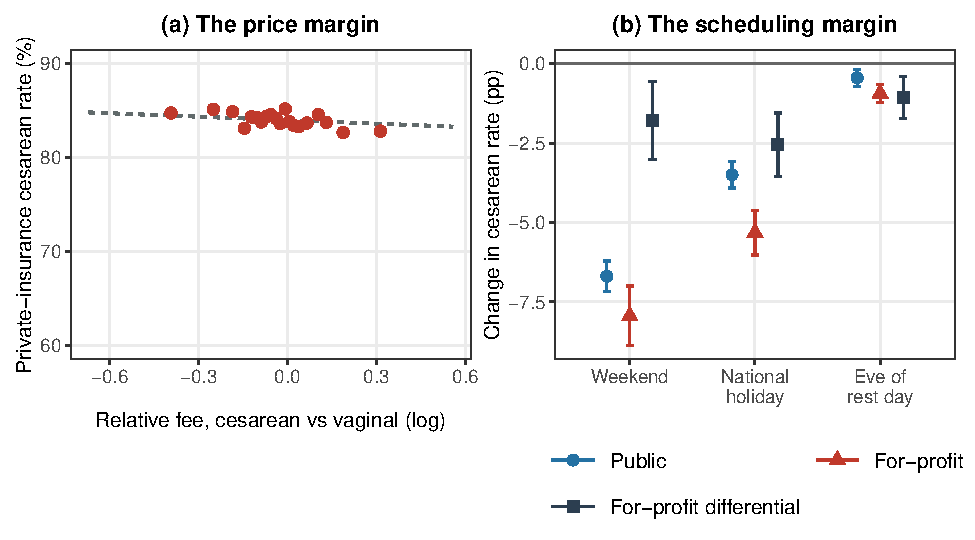
\includegraphics[width=\textwidth]{../analysis/output/graphs/fig_two_margins.pdf}
\caption{\textbf{Two margins of cesarean supply}}\label{fig:two_margins}
\fignotes{Panel (a): binscatter of the private-insurance cesarean rate on the log
economic fee gap across municipality-years with at least twenty private deliveries,
weighted by deliveries, after partialling out municipality and year fixed effects and
the municipal controls (log GDP per capita, private health-plan coverage, adequate
prenatal care, and obstetrician density); each point is an equal-mass bin over the
central 98 percent of the residualized fee gap, and the dashed line is the fitted
within-municipality slope, the coefficient of Table~\ref{tab:fees}, column 4. Panel (b):
weekend, national-holiday, and eve-of-rest-day coefficients, in percentage points,
with 95 percent confidence intervals from standard errors two-way clustered by
municipality and date. ``Public'' and ``For-profit'' are each sector's
own gradient from Equation~\eqref{eq:scheduling}; ``For-profit differential'' is the
within-municipality-day for-profit interaction from Equation~\eqref{eq:gradient}.}
\end{figure}

% =============================================================================
\section{Fees and the cesarean rate}\label{sec:notprice}
% =============================================================================

The obvious explanation for a high cesarean rate is that cesareans pay more. Per
delivery, on average, they do not. The correct comparison must credit the vaginal delivery
with the hourly labor-assistance fee it generates: 38 percent of vaginal
deliveries bill it, for 2.9 hours on average at about R\$420 per hour. Once it is
counted, the economic cesarean-minus-vaginal fee gap is negative in each of
Brazil's five largest states, by 18 to 38 percent, even though those states run
private-insurance cesarean rates of 78 to 90 percent. The economic vaginal fee is the mean, over all
vaginal deliveries, of the delivery fee plus any labor-assistance fee billed with
it, so it is the expected pay of a vaginal delivery, not the pay of every one:
vaginal deliveries that bill labor hours average R\$3,355, those that bill none
R\$1,778, below the cesarean fee of R\$1,939, and the vaginal delivery fee alone
averages R\$1,893 (\satab{tab:fee_per_hour}). The expected fee is the relevant
price because the comparison is made ex ante: when a cesarean is booked, the
physician does not know whether labor would have been long enough to bill. Part
of the spread is contractual rather than clinical, however. The share of vaginal
deliveries that bill labor assistance runs from 18 percent in S\~ao Paulo to 70
percent in Minas Gerais, and where it is billed often the delivery fee alone is
lower: in S\~ao Paulo and Rio de Janeiro, where it is rarely billed, the vaginal
delivery fee alone already exceeds the cesarean fee, while it is about equal to
it in Minas Gerais and below it in Paran\'a and Santa Catarina, where the hourly
code carries the difference. The expected fee therefore reflects insurers' and states' billing
norms as well as the length of labor. Counted by municipality-year rather than by
delivery, the gap is positive in most small municipalities, but 57 percent of
private deliveries take place where the cesarean pays less
(\satab{tab:descriptives}).

Per hour of the physician's time the ranking reverses. The cesarean fee, about R\$1,940, pays for roughly
an hour of surgery booked in advance, while the hours a vaginal delivery requires
are paid, when they are billed at all, at about R\$420 each. On average, a
vaginal delivery that occupies the physician for more than about 1.25 hours pays
less per hour than a cesarean, and for more than about 2.5 hours if the cesarean
itself takes two; the threshold lies between 1.2 and 1.6 hours in each of the
five largest states. It is about 1.7 hours for a vaginal delivery that bills
labor assistance and about 0.9 hours for one that bills none
(\satab{tab:fee_per_hour}). The labor hours that are billed already average 2.9,
and they are a floor on the time a vaginal delivery takes, since the deliveries
that bill none, 62 percent nationally and between 30 and 82 percent in the five
largest states, still take the physician's time. The price of time is therefore
not an alternative to a price explanation. The fee schedule pays the labor hours
that are billed, but not the on-call availability, the uncertain onset, or the
hours that go unbilled, and it is that unpriced part of physician time the
argument turns on. The per-hour ranking is itself set by the schedule, through
the hourly labor-assistance fee, which makes that fee a price lever on exactly
this margin; our data do not identify its effect. The model of
Appendix~\ref{sec:model} carries it as the convenience premium $\Pi$, the value of
converting unschedulable, calendar-blocking hours into a booked hour, and the
availability fee of Section~\ref{sec:background} is a market price for exactly
those hours: 4.5 percent of the deliveries in the claims carry no physician
delivery fee billed to the plan, an upper bound on those paid privately under such
an agreement, and our data do not observe what was paid. The fee data therefore
test something narrower than whether money matters: whether the relative fee per
procedure, the margin that fee-schedule policy moves, sustains the epidemic.
Nor do they see unobserved bonuses, ownership returns, or longer-run career
incentives.

Calibration answers that question without relying on our own estimates.
\citet{gruber1999physician} find that the cesarean rate rises with the
cesarean--vaginal fee differential at roughly four percentage points per
US\$1,000; re-estimating that response on corrected data, \citet{grant2009}
obtains about one percentage point per US\$1,000. Converted at our own fee levels,
the two bracket a response of roughly 0.7 to 2.9 percentage points per log point
of the fee gap. Applied to the 0.20 to 0.49 log point negative gap of Brazil's
largest states, they predict a movement of at most about a third of a percentage
point at the smaller response and 1.4 points at the larger, against a
for-profit--public gap of 36 points and a for-profit rate of about 81 percent. A
response to the relative procedure fee of the size the literature has documented
cannot carry an epidemic of this magnitude even at the larger of the two
responses, and the fact that the cesarean is, on average, the worse-paid procedure per delivery
precisely where cesarean rates are highest does not rest on any regression.

Our own estimates disagree with one another and do not discipline that
magnitude. Panel A of Table~\ref{tab:fees} estimates Equation~\eqref{eq:feegap},
regressing the private-insurance cesarean rate on the log economic fee gap across
municipality-years, weighting by deliveries and adding state or municipality fixed
effects and controls for income, plan coverage, prenatal care, and obstetrician
density. With the full controls the coefficient is 0.019 under state fixed
effects and $-0.013$ under municipality fixed effects, neither significant;
without the controls it is 0.049, significant at the 5 percent level, and
$-0.014$, significant at the 10 percent level. The two fixed-effect schemes fall
on opposite sides of the calibration. The within-municipality intervals place the
response below half a percentage point per log point of the fee gap, and so
exclude both of the literature's responses from below. The state-level estimate
without controls, 4.9 percentage points per log point, lies above the larger of
them, and the state-level intervals, resting on twenty-seven clusters, are about
three times wider and rule out little. Even that largest estimate, applied to the
0.49 log point gap, moves the cesarean rate by about 2.4 percentage points. Panel B uses the
year-to-year variation directly. State-level fee gaps swing by as much as 1.4 log
points from one year to the next, yet cesarean rates do not follow: in first
differences the coefficient is $-0.87$ percentage points per log point, and a
wild-cluster bootstrap over the twenty-two state clusters
\citep{cameron2008,webb2023} cannot distinguish it from zero ($p=0.32$); in levels
with state and year fixed effects it is likewise not distinguishable from zero
(bootstrap $p=0.17$). Two features limit what these regressions can
show. The billed fee gap is an average over insurers, contracts, and cases, so it
is endogenous to the local market, and swings of that size between consecutive
years suggest measurement error, which would bias the coefficient toward zero in
every specification.
And in none of the four specifications does the 95 percent interval fit inside a
region of plus or minus two percentage points per log point, so the regressions do
not establish that the response is small; the two state-level intervals contain
the canonical response of the literature (\satab{tab:feegap_ci}). The case rests
on the calibration alone; the regressions do not discipline the magnitude, and
none of them brings the relative fee anywhere near the 36-point gap. The 2015
court order to triple vaginal pay offers no additional test, since the agency
appealed and no rule was issued.

The Supplementary Appendix reports the confidence intervals, the equivalence
region and the calibration for the fee coefficient (\satab{tab:feegap_ci}), the
same regressions using the base rather than the economic vaginal fee
(\satab{tab:fee_base_econ}), the few-cluster bootstrap inference for the
state-year first difference (\satab{tab:fewcluster}), and the fees per hour of
physician time (\satab{tab:fee_per_hour}).

\begin{table}[H]
\centering
\caption{\textbf{Fees and the cesarean rate}}
\label{tab:fees}
\small\setlength{\tabcolsep}{5pt}
\resizebox{\ifdim\width>\linewidth \linewidth\else\width\fi}{!}{%
\begin{tabular}{lcccc}
\toprule
 & (1) & (2) & (3) & (4) \\
\midrule
\multicolumn{5}{l}{\emph{Panel A. Municipality-year levels}} \\
\addlinespace[2pt]
Log economic fee gap (cesarean minus vaginal) & 0.0488$^{**}$ & -0.0141$^{*}$ & 0.0190 & -0.0125 \\
 & (0.0235) & (0.0082) & (0.0236) & (0.0081) \\
\addlinespace[2pt]
\midrule
Municipal controls & No & No & Yes & Yes \\
State fixed effects & Yes & No & Yes & No \\
Municipality fixed effects & No & Yes & No & Yes \\
Year fixed effects & Yes & Yes & Yes & Yes \\
Observations & 5,198 & 5,198 & 4,706 & 4,706 \\
\midrule
\multicolumn{5}{l}{\emph{Panel B. State-year variation in the fee gap}} \\
\addlinespace[2pt]
 & \multicolumn{2}{c}{First differences} & \multicolumn{2}{c}{Levels} \\
\cmidrule(lr){2-3}\cmidrule(lr){4-5}
\addlinespace[2pt]
Change in the log fee gap & \multicolumn{2}{c}{-0.0087} & \multicolumn{2}{c}{} \\
 & \multicolumn{2}{c}{(0.0091)} & \multicolumn{2}{c}{} \\
\addlinespace[2pt]
Log fee gap & \multicolumn{2}{c}{} & \multicolumn{2}{c}{-0.0211} \\
 & \multicolumn{2}{c}{} & \multicolumn{2}{c}{(0.0164)} \\
\addlinespace[2pt]
Wild-cluster bootstrap $p$-value & \multicolumn{2}{c}{0.323} & \multicolumn{2}{c}{0.166} \\
\midrule
State fixed effects & \multicolumn{2}{c}{No} & \multicolumn{2}{c}{Yes} \\
Year fixed effects & \multicolumn{2}{c}{No} & \multicolumn{2}{c}{Yes} \\
State clusters & \multicolumn{2}{c}{22} & \multicolumn{2}{c}{22} \\
Observations & \multicolumn{2}{c}{189} & \multicolumn{2}{c}{208} \\
\bottomrule
\end{tabular}}
\begin{minipage}{\linewidth}\footnotesize
\textit{Notes:} The dependent variable is the share of private deliveries by
cesarean. The economic fee gap adds the separately billed hourly
labor-assistance fee to the vaginal delivery fee. Panel A estimates
Equation~\eqref{eq:feegap} on municipality-years with at least 20 private
deliveries, weighted by deliveries; municipal controls are log GDP per capita,
private health-plan coverage, adequate prenatal care, and obstetricians per 1,000
births; standard errors are clustered on the fixed-effect geography. Panel B
aggregates to state-years with more than 2,000 private deliveries and asks whether
year-to-year swings in the state fee gap move the cesarean rate; the levels column
adds state and year fixed effects. Because there are only twenty-two state clusters,
inference in both columns is complemented by a 9,999-draw Webb-weight wild-cluster
bootstrap. Standard errors, clustered by state, are reported in parentheses.
\newline
\footnotesize Significance levels: *** p$<$0.01, ** p$<$0.05, * p$<$0.10.
\end{minipage}
\end{table}


% =============================================================================
\section{Scheduling and the timing of cesareans}\label{sec:mechanism}
% =============================================================================

The natural onset of spontaneous labor does not respect the week, but the observed
delivery date can be changed through induction or prelabor cesarean scheduling.
Weekly differences in the observed cesarean rate therefore document calendar
sorting of deliveries.

\subsection{The for-profit calendar gradient}

Table~\ref{tab:main_gradient} reports our main estimating equation. In Panel B,
cesarean rates at for-profit establishments fall by 7.9 percentage points on
weekends and 5.3 points on national holidays, against public dips of 6.7 and 3.5
points. Most of the weekly gradient is therefore common to both sectors, and
weekly scheduling pervades Brazilian obstetrics.

Panel A isolates what is specific to the for-profit organizational model.
Estimating Equation~\eqref{eq:gradient}, which pools the two sectors so that the
municipality-by-date fixed effects absorb every shock they share on a given local
day, leaves a for-profit differential of a further 1.8 percentage points on
weekends and 2.5 points on holidays. This local contrast holds geography,
seasonality, and municipal holidays fixed and compares only the two ownership
types on the same day. The threat to it is that case-mix moves
differentially across sectors from weekday to weekend. Column 2 adds each cell's
own predetermined maternal composition, namely the shares of births in each
maternal age band, education category, race, and parity category, and leaves the
differential essentially unchanged, at 1.8 points on weekends and 2.4 on
holidays. Column 3 adds Robson-group shares, on 2014--2024, the years in which the
classification exists, and yields a further clinically
standardized comparison of 1.5 and 1.7 points. Because the Robson classification
encodes the onset of labor and gestational age, both of which scheduling itself
moves, we report it as a descriptive standardization rather than as the
preferred adjustment. The differential is therefore not an artifact of observed
case-mix. It does not distinguish physician convenience from ownership-specific
staffing, operating-room capacity, or scheduling protocols.

Columns 4 and 5 split the outcome into its two components and locate the
differential. It is concentrated in cesareans performed before labor began, the
only ones that scheduling can directly move, while the in-labor component moves
in the opposite direction, which is what displacement across days looks like.

A sector's share on a given day averages the shares of its establishments, so a
weekend fall in the cell can come from each hospital changing its practice or
from births moving, on weekends, toward hospitals that operate at lower cesarean
rates. \satab{tab:estab_gradient} separates the two by re-estimating
Equation~\eqref{eq:gradient} on establishment-day cells with
establishment-by-year fixed effects, so that the differential is identified only
from each establishment's own weekday-weekend variation, still against the other
sector in the same municipality-day. Within the establishment, the for-profit
weekend differential is 0.9 percentage points with birth weights and 1.3 with each
establishment's weight held at its mean daily births, against 1.8 on the same
births aggregated to the municipality-sector cell; the holiday differential is
1.3 and 1.8 against 2.5. Half or more of the headline differential, depending on
how establishments are weighted, is therefore a change of practice within the
hospital, and the rest is the reallocation of weekend births across hospitals. Both are features of how supply is organized, and
the same table shows the reallocation directly: on a weekend a for-profit
establishment is 8.7 percentage points less likely than a public one to record any
birth at all, its prelabor cesareans fall by 34 log points more, and its vaginal
births by 6.

\begin{table}[H]
\centering
\caption{\textbf{For-profit calendar gradient within the municipality-day}}
\label{tab:main_gradient}
\small\setlength{\tabcolsep}{4pt}
\resizebox{\ifdim\width>\linewidth \linewidth\else\width\fi}{!}{%
\begin{tabular}{lccccc}
\toprule
 & (1) & (2) & (3) & (4) & (5) \\
 & Cesarean & Cesarean & Cesarean & Prelabor & In-labor \\
 & share & share & share & cesarean share & cesarean share \\
\midrule
\multicolumn{6}{l}{\emph{Panel A. For-profit differential}} \\
\addlinespace[2pt]
For-profit $\times$ Weekend & -1.784$^{***}$ & -1.817$^{***}$ & -1.490$^{***}$ & -4.741$^{***}$ & 2.878$^{***}$ \\
 & (0.623) & (0.582) & (0.393) & (0.921) & (0.483) \\
\addlinespace[2pt]
For-profit $\times$ National holiday & -2.493$^{***}$ & -2.358$^{***}$ & -1.675$^{***}$ & -4.362$^{***}$ & 2.108$^{***}$ \\
 & (0.504) & (0.433) & (0.375) & (0.739) & (0.386) \\
\addlinespace[2pt]
For-profit $\times$ Eve of rest day & -1.049$^{***}$ & -0.997$^{***}$ & -0.818$^{***}$ & -1.343$^{***}$ & 0.339 \\
 & (0.336) & (0.325) & (0.278) & (0.438) & (0.256) \\
\addlinespace[2pt]
\midrule
Predetermined maternal composition & No & Yes & Yes & No & No \\
Robson-group shares & No & No & Yes & No & No \\
Municipality $\times$ date fixed effects & Yes & Yes & Yes & Yes & Yes \\
Sample & 2010--2024 & 2010--2024 & 2014--2024 & 2012--2024 & 2012--2024 \\
Observations & 5,038,183 & 5,038,183 & 3,591,268 & 4,300,868 & 4,300,868 \\
\midrule
\multicolumn{6}{l}{\emph{Panel B. Each sector's own gradient}} \\
\addlinespace[2pt]
 & \multicolumn{2}{c}{Public} & \multicolumn{2}{c}{For-profit} & \\
\cmidrule(lr){2-3}\cmidrule(lr){4-5}
\addlinespace[2pt]
Weekend & \multicolumn{2}{c}{-6.693$^{***}$} & \multicolumn{2}{c}{-7.940$^{***}$} & \\
 & \multicolumn{2}{c}{(0.245)} & \multicolumn{2}{c}{(0.479)} & \\
\addlinespace[2pt]
National holiday & \multicolumn{2}{c}{-3.511$^{***}$} & \multicolumn{2}{c}{-5.338$^{***}$} & \\
 & \multicolumn{2}{c}{(0.213)} & \multicolumn{2}{c}{(0.357)} & \\
\addlinespace[2pt]
Eve of rest day & \multicolumn{2}{c}{-0.446$^{***}$} & \multicolumn{2}{c}{-0.940$^{***}$} & \\
 & \multicolumn{2}{c}{(0.136)} & \multicolumn{2}{c}{(0.149)} & \\
\addlinespace[2pt]
\midrule
Municipality fixed effects & \multicolumn{2}{c}{Yes} & \multicolumn{2}{c}{Yes} & \\
Year fixed effects & \multicolumn{2}{c}{Yes} & \multicolumn{2}{c}{Yes} & \\
Observations & \multicolumn{2}{c}{3,611,665} & \multicolumn{2}{c}{1,426,518} & \\
\bottomrule
\end{tabular}}
\begin{minipage}{\linewidth}\footnotesize
\textit{Notes:} Municipality-date-sector cells, SINASC, weighted by births;
coefficients in percentage points. Panel A estimates
Equation~\eqref{eq:gradient}: municipality$\times$date fixed effects absorb every
shock common to the two sectors within a municipality-day, so the interactions are
the for-profit-specific gradient. Predetermined maternal composition is the cell's
share of births in each maternal age band, education category, race category, and
parity category. Robson-group shares standardize clinically but may respond to
scheduling, since the classification encodes labor onset and gestational age.
Columns 4--5 split the cesarean share into cesareans performed before and during
labor, on the years in which the timing indicator is recorded for more than 85
percent of cesareans. Panel B reports each sector's own gradient from
Equation~\eqref{eq:scheduling}, with municipality and year fixed effects.
Standard errors, two-way clustered by municipality and date, are reported in
parentheses.
\newline
\footnotesize Significance levels: *** p$<$0.01, ** p$<$0.05, * p$<$0.10.
\end{minipage}
\end{table}


Figure~\ref{fig:calendar} collects the calendar fingerprints. Panel (a) plots the
cesarean rate by day of the week and sector. At for-profit establishments the
rate is flat at 82 to 84 percent from Monday through Friday and drops sharply on
Saturday and Sunday; public establishments show the same shape at a lower level,
with the nonprofit sector in between. Panel (b) shows that for-profit cesareans
are rare overnight and spike between eight and eleven in the morning,
the operating-room block, while vaginal births are nearly uniform around the
clock. Half of all cesareans occur in weekday business hours, in both sectors
alike (50.1 percent for-profit and 50.9 percent public), against a benchmark of
29.8 percent under uniform timing, and only about a third of vaginal births do
(\satab{tab:business_hours}). The hour-of-day fingerprint is common to the two
sectors; what separates them is the weekend and holiday differential of
Table~\ref{tab:main_gradient}.

\begin{figure}[H]\centering
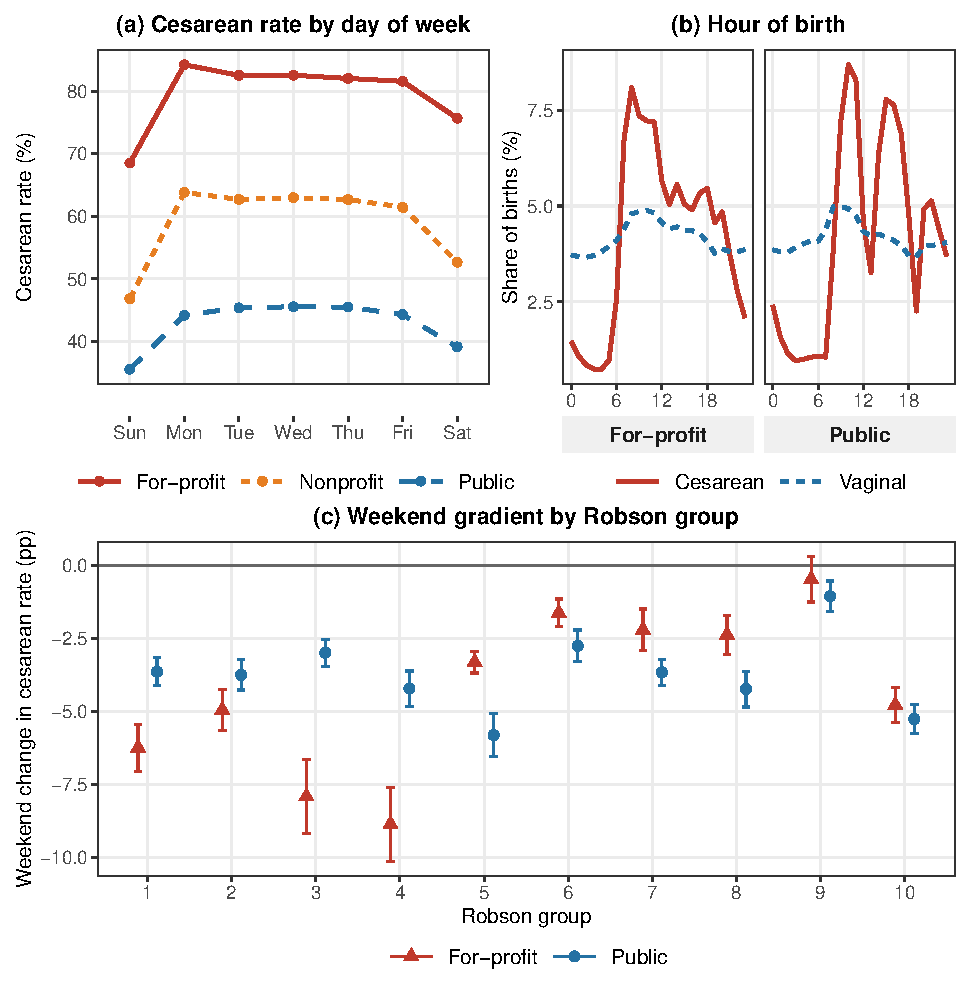
\includegraphics[width=\textwidth]{../analysis/output/graphs/fig_calendar_fingerprints.pdf}
\caption{\textbf{Calendar fingerprints of scheduled delivery}}\label{fig:calendar}
\fignotes{SINASC. Panel (a): cesarean rate by day of week and establishment
sector, 2010--2024. Panel (b): share of births by hour of birth, by delivery mode
and sector, 2010--2024. Panel (c): the weekend change in the cesarean rate,
in percentage points, estimated separately within each Robson group for each
sector from Equation~\eqref{eq:scheduling}, with 95 percent confidence intervals
from standard errors two-way clustered by municipality and date; Robson groups
are recorded from 2014, so panel (c) uses 2014--2024. Groups 1--2 are nulliparous
term singleton cephalic pregnancies, groups 3--4 their multiparous counterparts
without a previous cesarean, group 5 women with a previous cesarean, groups 6--9
breech, multiple, and abnormal-lie pregnancies, and group 10 preterm births.}
\end{figure}

\subsection{Where the dip lives: prelabor cesareans and low-risk births}

The components of the cesarean rate locate the mechanism.
Table~\ref{tab:prelabor_lowrisk} splits each sector's own weekend dip into
cesareans performed before labor began and cesareans performed during labor. At
for-profit establishments the weekend dip is 8.9 percentage points for prelabor
cesareans and a positive 1.9 points for in-labor cesareans. Scheduling operates
on prelabor surgery, and that is where the for-profit dip is concentrated; the
small positive in-labor term is displacement, as women who are not scheduled go
into labor and some convert. We use the timing indicator from 2012, when it is
recorded for most cesareans; from then on it is missing for about 7 percent of
for-profit and 10 percent of public cesareans, at rates that are essentially
identical on weekdays and weekends (\satab{tab:timing_missing}), and a cesarean
without it counts in neither component. At the level of the sector, the split is
therefore not an artifact of the indicator; within Robson group 1, where uncoded
cesareans are more frequent on weekdays, the balance does not hold. The
full timing split alongside the preterm (Robson group 10) comparison is in
\satab{tab:mechanism_checks}, and the day-of-week count series, in which cesarean
counts fall sharply on weekends while vaginal counts change little, is in
\safig{fig:daily_counts}.

The pattern extends to the least complicated pregnancies. Columns 5 and 6 of
Table~\ref{tab:prelabor_lowrisk} restrict attention to Robson groups 1 and 2,
first-time mothers at term with a single cephalic baby, the births for which a
cesarean is hardest to justify. The for-profit rate exceeds 80 percent on every
weekday and the weekend dip is 7.0 percentage points. Among Robson group 1 alone, first-time mothers in spontaneous
labor, the dip is still 6.0 points. Of that, 4.7 points are among cesareans coded
as performed during labor, which cannot come from prelabor scheduling; they
reflect intrapartum decisions and selection into who delivers on a weekend, and
show that the weekly calendar reaches even births that scheduling cannot directly
move. The remaining 1.3 points are among cesareans with no timing code, which the
register leaves in group 1 when the prelabor field is blank or marked as ignored.
Group-1 cesareans lack the code more often on weekdays than on weekends, so these
may include some cesareans performed before labor. \safig{fig:robson_dow} plots the day-of-week profile within these low-risk
groups, and \satab{tab:robson_validation} reports the timing indicator by Robson
group and tests the group-1 dip against the group-10 dip.

Panel (c) of Figure~\ref{fig:calendar} extends the exercise to the full Robson
classification, estimating each sector's own weekend gradient separately within
every group. The for-profit gradient is steepest, and clearly steeper than the
public one, in groups 1 through 4: term singleton cephalic pregnancies without a
previous cesarean, the deliveries in which the choice between labor and surgery
is genuinely open. The for-profit dip there runs from 5.0 to 8.9 percentage
points against 3.0 to 4.2 points in the public sector. Group 5, women with a
previous cesarean and the largest group of for-profit births (28.6 percent,
Table~\ref{tab:decomposition}), runs the other way: its for-profit dip, 3.3
points, is smaller than the public one, 5.8. A ceiling operates there.
For-profit establishments deliver 95 percent of these women by cesarean on
weekdays, against 80 percent in public hospitals, so a woman in this group who
reaches a weekend is still delivered by cesarean and the calendar can move the
date of her surgery but hardly its rate. The same ceiling flattens the
for-profit gradient in groups 6 through 9, breech, multiple, and abnormal-lie
pregnancies, which for-profit establishments deliver by cesarean 94 to 98 percent
of the time: there the for-profit dip is between 0.5 and 2.4 points, and in
groups 6 to 8 it is smaller than the public one. In group 10, preterm delivery, the two
sectors are statistically indistinguishable, at 4.8 and 5.3 points. The excess
weekend gradient of the for-profit sector is therefore concentrated in the groups
in which the choice between labor and surgery is still open, and absent both
where that choice is almost always surgery and among preterm births. We read this
as corroboration rather than as a placebo: Robson group membership is partly
determined by the same decisions we are studying, and preterm delivery is not
synonymous with unschedulable delivery.
\satab{tab:subgroup_gradients} reports the same contrast in the form of
Equation~\eqref{eq:gradient}, splitting births at 37 completed weeks, and adds a
split by maternal age.

\begin{table}[H]
\centering
\caption{\textbf{The weekend dip by delivery timing and clinical risk}}
\label{tab:prelabor_lowrisk}
\small\setlength{\tabcolsep}{4pt}
\resizebox{\ifdim\width>\linewidth \linewidth\else\width\fi}{!}{%
\begin{tabular}{lcccccc}
\toprule
 & (1) & (2) & (3) & (4) & (5) & (6) \\
 & \multicolumn{4}{c}{Components of the cesarean share} & \multicolumn{2}{c}{Cesarean share, low risk} \\
\cmidrule(lr){2-5}\cmidrule(lr){6-7}
 & Prelabor & In-labor & Prelabor & In-labor & Robson 1--2 & Robson 1 \\
\midrule
Weekend & -8.932$^{***}$ & 1.860$^{***}$ & -4.320$^{***}$ & -1.426$^{***}$ & -7.095$^{***}$ & -6.368$^{***}$ \\
 & (0.629) & (0.377) & (0.240) & (0.162) & (0.445) & (0.402) \\
\addlinespace[2pt]
\midrule
Sector & For-profit & For-profit & Public & Public & For-profit & For-profit \\
Municipality fixed effects & Yes & Yes & Yes & Yes & Yes & Yes \\
Year fixed effects & Yes & Yes & Yes & Yes & Yes & Yes \\
Observations & 1,201,804 & 1,201,804 & 3,099,064 & 3,099,064 & 730,120 & 439,712 \\
\bottomrule
\end{tabular}}
\begin{minipage}{\linewidth}\footnotesize
\textit{Notes:} Estimates of Equation~\eqref{eq:scheduling}, restricted to the
weekend indicator. Municipality-date cells, SINASC 2010--2024, weighted by births;
coefficients in percentage points. Columns 1--4 split the cesarean share of births
into cesareans performed before labor began and cesareans performed during labor.
Columns 5--6 restrict to Robson groups 1--2 (nulliparous, term, singleton,
cephalic) and to Robson group 1 alone, which requires spontaneous labor, so that
its cesareans are intrapartum by construction. Standard errors, two-way clustered
by municipality and date, are reported in parentheses.
\newline
\footnotesize Significance levels: *** p$<$0.01, ** p$<$0.05, * p$<$0.10.
\end{minipage}
\end{table}


\subsection{Long weekends and the displacement of scheduled cesareans}

If procedures are ordered around the calendar, they should be ordered around
blocks of rest, not merely around Sundays. We therefore ask a single economic
question with a single pre-specified exercise: are scheduled procedures moved
across dates so as to build longer blocks of leisure? The primary outcome is the
share of births delivered by prelabor cesarean, the primary window is the three
days on either side of a holiday, the primary sample is the eight fixed-date
national holidays over 2012 to 2024 (20 November, national only from 2024, is left
out), and the primary parameters are the
long-block coefficients and the sum of the pre-holiday event-time coefficients.
All of this was fixed before estimation, and we report the results whether or not
they support the hypothesis.

Classify each fixed-date national holiday by the day of the week on which it
falls. A holiday on a Wednesday is genuinely isolated: it yields one day
of rest attached to nothing. A holiday on a Monday or a Friday automatically
creates a three-day weekend. A holiday on a Tuesday or a Thursday is a
bridge: one further day off buys a four-day block, and Brazilian practice
is to take it. Holidays that fall on a Saturday or a Sunday add no workday of
rest and serve as a placebo. Extending Equation~\eqref{eq:gradient},
\begin{multline}
\text{Y}_{mds} = \lambda_{md} + \phi_{ms}
  + \gamma_I\,\text{ForProfit}_{s}\!\times\!\text{Isolated}_{d}
  + \gamma_3\,\text{ForProfit}_{s}\!\times\!\text{ThreeDay}_{d} \\
  + \gamma_B\,\text{ForProfit}_{s}\!\times\!\text{Bridge}_{d}
  + \sum_{w}\eta_w\,\text{ForProfit}_{s}\!\times\!\text{DOW}_{wd}
  + \sum_{h}\kappa_h\,\text{ForProfit}_{s}\!\times\!\text{Holiday}_{hd}
  + \varepsilon_{mds},
\label{eq:blocks}
\end{multline}
where the day-of-week interactions compare a holiday to ordinary days of the same
week day and the holiday-identity interactions compare a holiday to itself in
years when it falls elsewhere in the week. Without them, an apparent bridge effect
could be nothing more than a Tuesday effect or a Christmas effect. The
physician-leisure hypothesis predicts $\gamma_B$ more negative than $\gamma_I$ and
$\gamma_3$; we test $\gamma_B = \gamma_I$ and $\gamma_B = \gamma_3$ directly.

A dip on the holiday itself is not displacement. Displacement means procedures are
moved to adjacent dates, and shares cannot reveal it, because a share falls when
its numerator falls, when its denominator rises, or both, so we turn to counts.
Because every municipality-day carries exactly one for-profit and one
public cell once zeros are filled in, the municipality-by-date fixed effects of
Equation~\eqref{eq:gradient} are algebraically equivalent to differencing the two
sectors within the day. For each outcome $k$ in $\{$prelabor cesareans, in-labor
cesareans, vaginal births, total births$\}$ we estimate, on event time
$\ell = d - H$ measured from the holiday $H$,
\begin{equation}
Y^{k}_{md,\text{FP}} - Y^{k}_{md,\text{Pub}}
  = \alpha_m + \tau_{ym} + \sum_{w}\eta_w\,\text{DOW}_{wd}
  + \sum_{c}\sum_{\ell=-4}^{4}\theta^{k}_{c\ell}\,
    \mathbf{1}\{d \in W_c,\ d - H = \ell\} + e_{md},
\label{eq:event}
\end{equation}
where $c$ indexes the holiday type, $W_c$ its event windows, $\alpha_m$ are
municipality and $\tau_{ym}$ year-by-month fixed effects, non-window days are the
omitted category, and standard errors are two-way clustered by municipality and
date. Windows containing a second national holiday are dropped. If procedures are
pulled forward, $\sum_{\ell=-3}^{-1}\theta^{\text{prelabor}}_{\ell}$ is positive;
if they are merely retimed within the window, $\sum_{\ell=-3}^{3}\theta_{\ell}$ is
zero.

Neither prediction survives in our fixed-date holiday design. This does not
contradict \citet{melo2024}, who document both anticipation and postponement of
births around Carnival, with most displaced births occurring through cesarean
delivery: Carnival is a movable, unusually long, and socially salient holiday
and is excluded from Equation~\eqref{eq:blocks}. Our result is narrower: among
ordinary fixed-date national holidays, longer rest blocks do not generate larger
for-profit dips, and there is no pre-holiday bunching within the specified event
window. Table~\ref{tab:long_weekends}, Panel A, shows that a
bridge holiday does not produce a larger for-profit dip than an isolated one.
Columns 2 to 4 hold day of week and holiday identity fixed, so each coefficient
compares the same holiday falling on a weekday of the given type with the same
holiday falling on a weekend, the omitted category. On that comparison the
for-profit cesarean share is 0.8 percentage point lower on a bridge holiday, 1.4
on a three-day holiday, and 1.8 on an isolated Wednesday holiday, none of them
distinguishable from zero, and the tests of
$\gamma_B = \gamma_I$ and $\gamma_B = \gamma_3$ return $p$-values of 0.55 and
0.69. The prelabor cesarean share, the primary outcome, is between 3.4 and
4.0 points lower on every holiday type, and the equality tests again return
$p$-values above 0.7. The point estimates, if anything, run the wrong way: the
bridge coefficient is the smallest of the three. Column 1, which compares each
holiday type with ordinary days of the same weekday, also estimates holidays that
fall on a weekend and so add no workday of rest: their extra for-profit dip is
1.8 points, not distinguishable from zero (standard error 1.4).

Panel B of Table~\ref{tab:long_weekends} traces the counts, and there is no
pre-holiday excess of prelabor cesareans. Summing the event-time coefficients,
each measured in births per municipality-day, over the three days before a
bridge holiday gives $-0.47$ prelabor cesareans per municipality, a deficit
rather than the predicted bunching. Over the full seven-day window the deficit grows to $-1.24$
prelabor cesareans, $-0.31$ in-labor cesareans, $-0.27$ vaginal births and
$-2.01$ births in total, all relative to ordinary days of the same week day and
net of the public sector. Volume is not conserved within the window: for-profit
obstetric activity is depressed across the whole holiday period rather than
rearranged inside it. In the share versions reported in \satab{tab:displacement_robust},
the prelabor cesarean share falls by 9.5 points over the window while
the change in the overall cesarean share, $-0.3$ points (standard error 1.8), is
not distinguishable from zero, so what happens within the
window is a substitution of in-labor for prelabor cesareans on top of a general
reduction in deliveries. \safig{fig:displacement_event} plots the event-study
coefficients $\theta^{k}_{\ell}$ around bridge holidays for each count outcome.

Prelabor scheduling is avoided across an entire holiday period, which is
consistent with the calendar sorting the rest of the paper documents. But the
two sharper predictions of a physician-leisure account, that longer blocks of
rest generate larger dips and that procedures bunch immediately before the
block, are not supported. And because vaginal births and in-labor cesareans also
decline, some of what happens around holidays is a contraction of institutional
activity rather than the rearrangement of any individual's schedule. The calendar
evidence in this paper documents a supply-side pattern consistent with
scheduling, common to both sectors and stronger in the for-profit one; it does
not identify whose constraints generate it.
The contrast with Carnival suggests that displacement may depend on the duration
and social salience of the holiday rather than on the existence of an attached
rest day alone.

\begin{table}[H]
\centering
\caption{\textbf{Long weekends and the displacement of scheduled cesareans}}
\label{tab:long_weekends}
\small\setlength{\tabcolsep}{5pt}
\resizebox{\ifdim\width>\linewidth \linewidth\else\width\fi}{!}{%
\begin{tabular}{lcccc}
\toprule
 & (1) & (2) & (3) & (4) \\
 & Cesarean & Cesarean & Prelabor cesarean & In-labor cesarean \\
 & share & share & share & share \\
\midrule
\multicolumn{5}{l}{\emph{Panel A. Holiday taxonomy, for-profit differential}} \\
\addlinespace[2pt]
For-profit $\times$ Bridge holiday (Tue/Thu) & -2.427$^{**}$ & -0.826 & -3.389$^{*}$ & 2.522$^{***}$ \\
 & (1.124) & (1.624) & (1.801) & (0.749) \\
\addlinespace[2pt]
For-profit $\times$ Three-day holiday (Mon/Fri) & -3.156$^{***}$ & -1.354 & -3.618$^{*}$ & 2.543$^{**}$ \\
 & (1.047) & (1.595) & (1.849) & (0.988) \\
\addlinespace[2pt]
For-profit $\times$ Isolated holiday (Wed) & -3.571$^{**}$ & -1.822 & -4.042$^{*}$ & 1.911$^{**}$ \\
 & (1.458) & (1.921) & (2.097) & (0.827) \\
\addlinespace[2pt]
For-profit $\times$ Weekend holiday (placebo) & -1.815 &  &  &  \\
 & (1.403) &  &  &  \\
\addlinespace[2pt]
\midrule
$p$-value: Bridge $=$ Isolated & 0.521 & 0.545 & 0.703 & 0.359 \\
$p$-value: Bridge $=$ Three-day & 0.635 & 0.688 & 0.876 & 0.979 \\
\addlinespace[2pt]
For-profit $\times$ day-of-week & Yes & Yes & Yes & Yes \\
For-profit $\times$ holiday identity & No & Yes & Yes & Yes \\
Municipality $\times$ date fixed effects & Yes & Yes & Yes & Yes \\
Observations & 4,256,023 & 4,256,023 & 4,256,023 & 4,256,023 \\
\midrule
\multicolumn{5}{l}{\emph{Panel B. Displacement around bridge holidays (counts, for-profit minus public)}} \\
\addlinespace[2pt]
 & Prelabor & In-labor & Vaginal & Total \\
 & cesareans & cesareans & births & births \\
\addlinespace[2pt]
Pre-holiday excess, $\sum_{\ell=-3}^{-1}\theta_\ell$ & -0.4684$^{*}$ & -0.2098$^{**}$ & -0.0774$^{**}$ & -0.8315$^{**}$ \\
 & (0.2589) & (0.0899) & (0.0319) & (0.3641) \\
\addlinespace[2pt]
Window total, $\sum_{\ell=-3}^{+3}\theta_\ell$ & -1.2410$^{***}$ & -0.3081$^{**}$ & -0.2723$^{***}$ & -2.0053$^{***}$ \\
 & (0.3831) & (0.1305) & (0.0699) & (0.5099) \\
\addlinespace[2pt]
\midrule
Day-of-week controls & Yes & Yes & Yes & Yes \\
Municipality fixed effects & Yes & Yes & Yes & Yes \\
Year $\times$ month fixed effects & Yes & Yes & Yes & Yes \\
Observations & 1,215,744 & 1,215,744 & 1,215,744 & 1,215,744 \\
\bottomrule
\end{tabular}}
\begin{minipage}{\linewidth}\footnotesize
\textit{Notes:} SINASC 2012--2024, the years in which the prelabor indicator is
recorded for about 85 percent of cesareans or more. Panel A: municipality-date-sector
cells with at least one birth, weighted by births; movable holidays are excluded.
Each fixed-date national holiday is classified by the day of week on which it falls.
Columns 2--4 add for-profit $\times$ holiday-identity indicators, so the weekend-
falling holiday is the omitted category and the coefficients are identified within
holiday and within day of week. Coefficients are in percentage points.
Panel B: balanced municipality-date panel of the two sectors, counts in births,
event time $\ell$ measured in days from the holiday, non-window days omitted,
municipality and year-month fixed effects with day-of-week controls;
$\theta_\ell$ is the for-profit minus public difference on event day $\ell$
relative to an ordinary day of the same week day. The observation count is the
municipality-days of the balanced panel and is common to the four columns.
Standard errors, two-way clustered by municipality and date, are reported in parentheses.
\newline
\footnotesize Significance levels: *** p$<$0.01, ** p$<$0.05, * p$<$0.10.
\end{minipage}
\end{table}


\subsection{Organizational capacity and weekend scheduling}\label{sec:capacity}

Establishments that can staff a weekend may behave differently. Linking each
for-profit birth to its establishment in the national facility registry, we
measure the establishment's obstetric bed count and annual delivery volume in
the previous calendar year, so that both are predetermined with respect
to current scheduling, and interact them with the weekend and holiday indicators
across for-profit establishments, absorbing establishment-by-year and
municipality-by-date fixed effects. The calendar gradient is flatter at larger
and higher-volume establishments. The two measures are related but not
collinear: across establishment-years their logarithms correlate at 0.48, and
net of the fixed effects the two weekend interactions correlate at 0.56. With
date rather than municipality-by-date fixed effects and both entered, a log point
of annual deliveries attenuates the weekend dip in the prelabor cesarean share by
1.49 percentage points (standard error 0.34) and a log point of obstetric beds by
0.47 points (standard error 0.35), so the variation across municipalities favors
delivery scale. The municipality-by-date fixed effects cut the residual standard
deviation of the bed interaction by a third and that of the scale interaction by
half. Entered together under them, the specification fixed in advance for the
multiple-testing adjustment, a log point of annual deliveries attenuates the dip
by 0.64 points (standard error 0.41) and a log point of beds by 0.58 points
(standard error 0.38): jointly significant ($p=0.02$), neither distinguishable
from zero on its own. Entered without the bed count, the delivery-scale
interaction is 1.3 to 1.4 points and precisely estimated, whether it stands
beside registered obstetricians, contracted obstetrician hours, or beds per
delivery, and the bed count entered without delivery scale attenuates the dip by
0.80 points (standard error 0.35). The attenuation therefore tracks the scale of
the service, within municipality-days as well as across them; within
municipality-days the data cannot apportion it between beds and volume, because
too little variation is left, not because the two move together. \satab{tab:org_capacity} reports these regressions
and \satab{tab:org_capacity_valid} reports them under alternative capacity
measures and samples. The second table also carries the validation finding behind
our choice of beds over registered physicians as the capacity measure. Among
for-profit hospitals with at least fifty deliveries, 14 percent register no
obstetrician at all in the CNES register of professionals. Brazilian obstetricians hold
their registry bond at their own practice rather than at the delivery hospital,
so the count reflects registration rather than the on-call roster. This comparison does not separate the individual physician's calendar
from the hospital's staffing constraint, since both predict a smaller weekend
gradient at larger establishments: a large obstetric service supplies call
coverage and, at the same time, independence from any one physician's schedule. The
pattern of point estimates is consistent with organizational redundancy
attenuating the calendar gradient, in line with evidence that maternity-ward staffing, crowding,
and available capacity alter procedure use
\citep{maibom2021,facchini2022,bachner2024,bensnes2026}; because facility scale
is not randomly assigned, we do not interpret the interaction as the causal
effect of capacity. It is nonetheless the margin a policy could act on.

A second capacity account comes from \citet{elejalde2021} and is the leading
alternative to reading our gradient as a calendar phenomenon. In their Chilean
setting, hospitals paid the same price for either mode of delivery still raised
the cesarean rate, because scheduling lets a hospital move deliveries off weeks it
expects to be crowded and take more deliveries in total. Two implications of that
account are testable in our data, and we fixed both before estimating them;
\satab{tab:demand_smoothing} reports the results. The first is pull-forward: the
prelabor cesarean share of a week should rise with the demand the establishment
expects in the following week, which we measure as the leave-one-out mean of its
own births in that week of the year across all other years. It does not: the
coefficients are small, of either sign, and none is distinguishable from zero.
That test is weak, since out of sample the forecast recovers only 0.05 log points
of realized relative demand per log point, so it bounds only large responses. The
second implication is better powered. If scheduling levels the flow of deliveries,
an establishment-year that schedules more should have a smoother weekly flow.
Within establishments there is no sign of levelling: the point estimate goes the
other way, a higher prelabor cesarean share going with a higher variance-to-mean
ratio of weekly births (0.31 log points per unit of the share, standard error
0.16), significant only at the 10 percent level and not after the family
adjustment below. The mechanism that operates without a price gap in Chile is
therefore not visible here.

Because this section and Section~\ref{sec:cost} each report several tests, the
Supplementary Appendix groups the hypotheses into pre-specified families and
reports Holm-Bonferroni adjusted $p$-values \citep{holm1979} and
Benjamini-Hochberg $q$-values \citep{benjamini1995}
within each (\satab{tab:multiple_testing}). The adjustment leaves the
within-municipality-day calendar gradient and the outcome differences
significant; it removes the individual significance of the long-weekend
coefficients, which we do not read as evidence, and none of the
demand-smoothing estimates is significant after it. The
Supplementary Appendix also reports the municipality-level heterogeneity of the
dip by obstetrician density and by maternal education (\satab{tab:heterogeneity})
and a contrast of physician-owned cooperative insurers with insurer-run plans
(\satab{tab:modality}). The dip is larger where
obstetricians are scarce relative to births and is smaller for more-educated
mothers, 7.2 against 11.2 percentage points, partly because their weekday rate
is already closer to its ceiling. This pattern does not support a simple model in which
greater maternal ability to schedule drives the aggregate gradient, although it
cannot rule out unobserved maternal preferences or joint physician--patient
scheduling decisions.


% =============================================================================
\section{Gestational-age and billed-amount margins}\label{sec:cost}
% =============================================================================

\paragraph{The gestational-age margin.} Scheduling a cesarean means performing
it before labor, and to be sure of preceding labor the physician must book it
before the natural rise in the delivery hazard around week 39. The mechanical
consequence is a shift of births to earlier gestational ages.
\safig{fig:gestation}, panel (a), shows both sectors peaking at 39 weeks with the
for-profit distribution sitting earlier: 41 percent of for-profit births fall at 37
or 38 weeks against 26 percent of public births, and 17 percent at 40 or 41 weeks
against 32 percent. Panel (b) orders the same shift by delivery timing within the
for-profit sector, prelabor cesareans earliest, in-labor cesareans next and vaginal
births latest. Table~\ref{tab:health} estimates that
for-profit births are 12.2 percentage points more likely to be early-term
(37--38 weeks) than public births, after controlling for maternal age,
education, and race with municipality and year fixed effects. The estimate is
associational. Sector and delivery mode are chosen, and the maternal controls
cannot absorb differences in pregnancy risk, assisted reproduction, prior
cesarean, or the measurement of gestational age, so the early-term coefficient
is a descriptive sector difference and is not interpreted as the causal effect
of prelabor scheduling. The calendar reaches gestational age inside the design of
Equation~\eqref{eq:gradient} as well. On a weekend the share of for-profit births
at 37--38 weeks falls 1.3 percentage points more than the public share, and 0.7
points among Robson 1--2 births, significant only at the 10 percent level
(\satab{tab:estab_gradient}, Panel B), so the early-term births of the for-profit
sector concentrate on the weekdays on which surgery is booked. This is calendar
ordering, not the effect of scheduling on any one pregnancy. Early-term delivery is the margin the clinical
literature links to higher neonatal respiratory morbidity and intensive-care use
\citep{tita2009}, and quasi-experimental work links non-indicated and
early cesareans to worse newborn health \citep{costaramon2018,borra2019}. For-profit
births show lower low-birthweight and low-Apgar rates, consistent with the better
resources and healthier mothers of that sector. Among Robson 1--2 births at term,
the pregnancies the two sectors share most closely, the advantage shrinks from 3.5
to 1.1 points in low birthweight and from 0.6 to 0.4 in low Apgar
(Table~\ref{tab:health}, columns 5--6). The descriptive health margin
associated with the for-profit delivery system is a shift toward early-term
birth. An ecological check relating early-term shifting to neonatal hospital
use, whose early-term coefficients are not distinguishable from zero, is in
\satab{tab:neonatal_suggestive}.

The shift is not costless: \citet{tita2009} find that elective delivery at
37--38 weeks, rather than at 39, raises the rate of adverse neonatal outcomes,
including respiratory morbidity and intensive-care admission. We do not convert
our associational sector gap into a count of harmed newborns, because the
mapping from a chosen sector to a causal harm requires a design we do not have.
The direction, however, is what both the clinical literature \citep{tita2009} and
quasi-experimental evidence on non-indicated and early cesareans
\citep{costaramon2018,borra2019} would predict, and it locates the health cost of
the for-profit delivery pattern in earlier, riskier births rather than in spending.

\begin{table}[H]
\centering
\caption{\textbf{For-profit--public differences in early-term birth and newborn outcomes}}
\label{tab:health}
\small\setlength{\tabcolsep}{5pt}
\resizebox{\ifdim\width>\linewidth \linewidth\else\width\fi}{!}{%
\begin{tabular}{lcccccc}
\toprule
 & (1) & (2) & (3) & (4) & (5) & (6) \\
 & \multicolumn{2}{c}{Early-term birth} & Low birthweight & Five-minute & Low birthweight & Five-minute \\
 & \multicolumn{2}{c}{(37--38 weeks)} & ($<$2500g) & Apgar $<$ 7 & ($<$2500g) & Apgar $<$ 7 \\
\cmidrule(lr){2-3}\cmidrule(lr){4-4}\cmidrule(lr){5-5}\cmidrule(lr){6-6}\cmidrule(lr){7-7}
For-profit establishment & 14.51$^{***}$ & 12.18$^{***}$ & -3.47$^{***}$ & -0.63$^{***}$ & -1.06$^{***}$ & -0.39$^{***}$ \\
 & (0.78) & (0.77) & (0.61) & (0.06) & (0.12) & (0.03) \\
\addlinespace[2pt]
\midrule
Maternal controls & No & Yes & Yes & Yes & Yes & Yes \\
Sample & All & All & All & All & Robson 1--2, term & Robson 1--2, term \\
Municipality fixed effects & Yes & Yes & Yes & Yes & Yes & Yes \\
Year fixed effects & Yes & Yes & Yes & Yes & Yes & Yes \\
Observations & 23,560,481 & 22,437,099 & 22,859,931 & 22,564,401 & 5,828,472 & 5,780,468 \\
\bottomrule
\end{tabular}}
\begin{minipage}{\linewidth}\footnotesize
\textit{Notes:} Birth-level regressions, SINASC 2010--2024, for-profit vs
public establishments; coefficients in percentage points. Columns 1--2 use the
births with a recorded gestational age: 3 percent of 2010 births, 57 percent of 2011
births, and at least 92 percent in every year from 2012. Maternal controls:
age, age$^2$, education, race. Mothers differ across sectors, so the
early-term coefficient is an associational difference between establishment
sectors and is not interpreted as the causal effect of prelabor scheduling.
Columns 5--6 restrict to Robson groups 1--2 (nulliparous, term, singleton,
cephalic; recorded from 2014) at 37 or more weeks, where selection across
sectors is smallest.
Standard errors, clustered by municipality, are reported in parentheses.
\newline
\footnotesize Significance levels: *** p$<$0.01, ** p$<$0.05, * p$<$0.10.
\end{minipage}
\end{table}


\paragraph{The billed-amount margin.} Billed amounts do not favor the cesarean
either. Summing every item billed under each delivery hospitalization, a
cesarean and a vaginal delivery generate similar gross billed amounts: the mean
cesarean bills about 1 percent less and the median about 4 percent more
(\satab{tab:cost}). These are charged amounts, not the
negotiated prices ultimately paid. Cesareans are therefore not obviously more
lucrative to bill per delivery; consistent with the fee analysis of
Section~\ref{sec:notprice}, the epidemic's margin lies in earlier, riskier births
rather than in higher billed amounts per delivery.

\paragraph{The size of the margin.} Table~\ref{tab:decomposition} decomposes the
36 percentage-point for-profit--public gap over Robson clinical groups. Only 27
percent reflects differences in case-mix; the remaining 73 percent is
within-group practice style, women in the same clinical group managed
differently. That most of the
gap is practice style rather than patient composition echoes the finding, in the
literature on geographic variation in health care, that supply-side practice
patterns dominate patient case-mix \citep{finkelstein2016,molitor2018}. For
cesarean delivery specifically, \citet{fischer2026} instrument where a mother
delivers with closures of a county's last obstetric unit and find that a one
percentage point higher cesarean rate in the delivery county raises her own
probability of a cesarean by about one point, so the delivery environment passes
through nearly one for one. Reweighting each
hospital's own group-specific rates to a common Robson distribution, the
comparison the World Health Organization's current guidance recommends, leaves the standard deviation of
cesarean intensity across for-profit hospitals at 14 percentage points.
Municipality-by-year fixed effects, predetermined maternal composition and obstetric
capacity together bring it to 6.3 points, 44 percent of where it started. Two for-profit hospitals delivering in the
same municipality and year differ by 12 percentage points on average in the
standardized rate (\satab{tab:estab_practice_style}).
Benchmarking
each municipality's weekday cesarean propensity against its own weekend rate
places about 35,000 for-profit weekday cesareans per year above that mechanical
benchmark, about one in eleven of the 380,000 cesareans the sector performs on weekdays in
an average year. This counts cesareans above the own-municipality
weekend rate; it does not separate procedures that would not have occurred from
those merely shifted off the weekend, and the weekend rate itself need not be the
clinical optimum.\footnote{This benchmark and the headline coefficient answer
different questions. The benchmark prices the sector's
whole gross weekend gradient against its own weekend rate: municipality-year by
municipality-year it gives the 35,000 of the text, and the regression gradient of
7.9 percentage points applied to 463,000 for-profit weekday births a year gives a
similar 37,000. They differ because the count applies each municipality-year's own
weekday-weekend gap to its own weekday births, while the regression averages the
gradient across municipalities and holds holidays and eves fixed. Equation~\eqref{eq:gradient} instead nets out the weekly scheduling
common to both sectors and prices only the for-profit differential of 1.8 points,
which on the same base is about 8,000 a year. The larger figure is the size of
weekday scheduling in this sector, the smaller one the part specific to for-profit
ownership.} Consistent with the
picture that most privately insured cesareans are elective, about four in five (77 to
81 percent in each year) carry no primary diagnosis in the claims other than a
delivery-outcome code or none at all (\satab{tab:no_indication}).

\begin{table}[H]\centering
\caption{\textbf{Decomposing the for-profit--public cesarean gap (Kitagawa, Robson groups)}}
\label{tab:decomposition}
\small
\small\setlength{\tabcolsep}{4pt}\resizebox{\ifdim\width>\linewidth \linewidth\else\width\fi}{!}{%
\begin{tabular}{lcccc}
\toprule
Robson group & Share for-profit (\%) & Share public (\%) & Cesarean for-profit (\%) & Cesarean public (\%) \\
\midrule
01 & 14.6 & 19.8 & 65.8 & 35.1 \\
02 & 22.1 & 10.4 & 89.0 & 55.5 \\
03 & 9.6 & 25.5 & 39.9 & 15.0 \\
04 & 9.4 & 8.8 & 75.6 & 38.0 \\
05 & 28.6 & 19.8 & 94.6 & 78.4 \\
06 & 1.9 & 1.2 & 94.6 & 88.2 \\
07 & 2.3 & 1.9 & 93.6 & 84.8 \\
08 & 2.7 & 2.1 & 93.6 & 80.0 \\
09 & 0.2 & 0.2 & 98.0 & 96.7 \\
10 & 8.5 & 10.3 & 76.9 & 42.8 \\
\midrule
\multicolumn{5}{l}{Gap 36.2pp $=$ case-mix 10.0pp (27\%) $+$ practice style 26.3pp (73\%)} \\
\bottomrule
\end{tabular}
}
\begin{minipage}{\linewidth}\footnotesize
\textit{Notes:} SINASC 2014--2024 (Robson classification available from 2014). Kitagawa decomposition \citep{kitagawa1955} of the for-profit--public cesarean gap into Robson-group composition and within-group rate differences.
\end{minipage}
\end{table}


% =============================================================================
\section{Conclusion}\label{sec:conclusion}
% =============================================================================

Brazil's for-profit maternity sector performs cesareans at one of the highest rates
recorded in any health system, and the standard version of the economic
explanation, that the procedure pays more, does not fit. Measured with the actual
fees, cesareans do not pay more per delivery than the average vaginal delivery
where the epidemic is worst, and the response to the relative fee documented in the
literature is far too small to account for a rate of this size. Per hour of
physician time, however, the cesarean is the better-paid procedure: the schedule
pays labor hours when they are billed, but not the on-call availability that a
vaginal delivery demands. The observed
patterns are consistent with cesareans being used to convert an
unschedulable, long, calendar-blocking event into a shorter, schedulable
procedure. Cesarean use carries the calendar fingerprints of that logic. It
clusters on weekdays and in business hours and dips on weekends and holidays,
and the dip is concentrated in surgery booked before labor, although sizable
intrapartum differences remain among the lowest-risk mothers. Within the same
municipality and day, the for-profit cesarean rate falls 1.8 percentage points
more on weekends than the public one, and for-profit births are more often
early-term. These
patterns are consistent with supply-side convenience scheduling, though our data
cannot isolate the attending physician's own time from hospital staffing,
operating-room
capacity, and scheduling protocols, and two results mark that boundary directly.
Among ordinary fixed-date national holidays, long weekends do not deepen the dip
relative to isolated holidays, and prelabor cesareans do not bunch in the days
before a long block, so the specific predictions of a physician-leisure account go
unconfirmed. And around holidays vaginal births fall alongside prelabor cesareans,
which is what a contraction of institutional activity, rather than the
rearrangement of an individual's schedule, would produce.

\citet{elejalde2021} reach a version of the same point from the other direction:
in Chile an incentive to operate survived the removal of the price differential
altogether, through the schedulability of the procedure. Here the differential
runs the other way and the incentive survives that too, but the margin it leaves
behind is not theirs. Their hospitals use scheduling to level demand across weeks,
whereas the Brazilian pattern is weekly, and the establishments that schedule most
show no smoother weekly flow.

The evidence identifies calendar sorting and a tightly controlled
for-profit--public differential; it does not identify the total number of
cesareans or neonatal outcomes caused by scheduling.

If, as the combined evidence suggests, an important margin is the organization of
obstetric time rather than the observed fee differential, the levers most worth
testing are organizational rather than financial, and three directions follow
from the analysis. The results identify organizational margins worth testing in future
policy interventions; they do not show that organizational interventions will
reduce cesareans. The first acts on the convenience premium directly: detaching the
delivery from a single attending physician's calendar, through laborist or
shift-based on-call coverage and midwife-led continuity of care, socializes the
cost of unschedulable time that the premium capitalizes. It should not be
expected to remove the weekly gradient itself. Among publicly paid births only
about 9 percent of women are delivered by the professional who followed their
pregnancy, against about 77 percent among privately paid ones
\citep{domingues2014}, yet public hospitals show most of the gradient too. We
therefore read its common part as reflecting how hospitals book surgery and staff
weekends, and the for-profit increment as what detaching the delivery from one
physician's calendar would target. The second changes how
care is organized rather than how it is priced. Most of the for-profit--public
gap is supply-side practice style rather than case-mix, and a physician's
practice style adjusts to the environment she practices in:
\citet{molitor2018} estimates that the environment accounts for 60 to 80 percent
of regional variation in physician behavior, and \citet{fischer2026} show that
the delivery environment passes through nearly one for one into a mother's own
cesarean probability \citep[see also][]{finkelstein2016,cutler2019}. Salaried or
vertically integrated arrangements in place of the private-office fee-for-service
model therefore act on the margin that actually varies, whereas relative-price
reforms act on one whose documented magnitude in childbirth is too small to
matter here \citep{gruber1999physician,grant2009}. This is a change in the
structure of pay, not in relative prices. The fee evidence concerns the price of
one mode of delivery relative to the other, whereas a salaried or shift-based
obstetrician is paid the same whichever mode is chosen and whenever the birth
occurs. The reform therefore removes from the attending physician the cost of
unschedulable time, the convenience premium of the model, and leaves the fee gap
untouched. The third ties regulation to gestational and
delivery outcomes rather than to prices, since it is delivery practice, and not
the price of a delivery, that the evidence links to newborn health
\citep{costaramon2018,card2023,borra2019}. The fee
evidence gives no reason to expect much from the relative per-procedure fee. The
hourly labor-assistance fee, which sets the per-hour ranking, is the one fee lever
that acts on the price of time, and our data do not evaluate it. The calendar
evidence points to the organization of obstetric time as a promising policy
margin.

How far these conclusions travel depends on which part of the setting one carries
along. Three features of Brazil's privately insured maternity care are extreme rather than typical:
a cesarean rate above 80 percent that leaves little room for the margin to move further, a
private-office fee-for-service model in which one obstetrician follows a patient
through pregnancy and expects to attend the delivery personally, and a fee schedule
in which the vaginal delivery is, on average, the better-paid procedure per
delivery once labor assistance is counted. Our magnitudes are specific to that configuration, and the
negative per-delivery fee gap in particular is unusual enough that the limited
role we find for the relative fee should not be read as a general statement about
how obstetricians respond to prices. The mechanism and the
diagnostic are portable. Wherever a delivery binds a single physician's
calendar for an uncertain interval and a cesarean does not, the convenience premium
exists and should leave the same calendar signature, and the weekday-weekend
gradient measured within a market and a day is a cheap test that any system with
dated birth records can run. Whether that premium is large enough to move practice
elsewhere is an empirical question our data cannot settle for other countries.

% =============================================================================
% Declarations, in the Elsevier/JHE order: CRediT, competing interests, funding,
% data availability, generative-AI use. All appear before the references.
% =============================================================================
\section*{CRediT authorship contribution statement}
% Roles confirmed by Fredie on 2026-09-07 and final. Do not reallocate.
\textbf{Fredie Didier:} Conceptualization, Methodology, Software, Formal
analysis, Data curation, Writing -- original draft, Writing -- review \&
editing. \textbf{Vinicius Mendes:} Conceptualization, Methodology, Writing --
review \& editing. \textbf{Pablo Castro:} Conceptualization, Methodology,
Writing -- review \& editing. \textbf{Lucas Emanuel:} Conceptualization,
Methodology, Writing -- review \& editing.

\section*{Declaration of competing interest}
The authors declare that they have no known competing financial interests or
personal relationships that could have appeared to influence the work reported
in this paper.

\section*{Funding}
This research did not receive any specific grant from funding agencies in the
public, commercial, or not-for-profit sectors.

\section*{Data availability}
The data underlying this article are drawn entirely from public administrative
sources. The TISS private-insurance hospital claims are published by the ANS on
its open-data portal \citep[\url{https://dadosabertos.ans.gov.br/FTP/PDA/TISS/}]{data_ans_tiss}. The
SINASC live-birth records are maintained by the Ministry of Health
\citep{data_sinasc} and are obtained from the Ministry's DATASUS repository
(\url{https://datasus.saude.gov.br}). The CNES facility and professional registries
\citep{data_cnes} and the IEPS municipal panel \citep[\url{https://iepsdata.org.br}]{data_ieps} are likewise public.
The Parto Adequado Phase-2 participating-hospital list is published by the
ANS \citep{data_parto_adequado}.
A draft replication package is available to editors and referees and will be
deposited in a trusted open repository prior to acceptance. It contains a master
script, code for downloading and transforming the source data, analysis code,
software and package versions, expected runtime, data citations, and a
program-to-output inventory.

\section*{Declaration of generative AI and AI-assisted technologies in the
manuscript preparation process}
\begin{sloppypar}
During the preparation of this work the authors used large-language-model
assistants (Claude, Anthropic; ChatGPT, OpenAI) to draft and edit portions of
the analysis code and the manuscript text. After using these tools, the authors
reviewed and edited the content as needed, verified all results against the
source data, and take full responsibility for the content of the published
article.
\end{sloppypar}

% =============================================================================
% References come before the appendices, per the Elsevier/JHE layout. The
% essential appendices (A model, B data) follow; the Supplementary Appendix
% (additional results and robustness) is a separate document,
% latex/supplement.tex, submitted as online supplementary material.
% =============================================================================
\bibliographystyle{plainnat-rev}
\bibliography{refs}

\appendix
% Number appendix tables/figures by their appendix section (A.1, B.1 ...),
% so a cross-reference makes clear which appendix an exhibit lives in.
\numberwithin{table}{section}
\numberwithin{figure}{section}

% =============================================================================
% appendix.tex — the essential appendix, \input by paper.tex after \appendix.
%   Appendix A: the model (via % =============================================================================
% model.tex — A simple model of delivery-mode choice and physician time.
% % =============================================================================
% model.tex — A simple model of delivery-mode choice and physician time.
% \input{model} from paper.tex. Delivers the five predictions tested in the
% empirical sections (P1-P5) and the policy corollary.
% =============================================================================

\section{A simple model of delivery-mode choice and physician time}
\label{sec:model}

\subsection{Setup}

A physician attends a pregnancy whose labor, absent intervention, begins at a
random time $\tilde{t}$ distributed (approximately) uniformly over the days and
hours of the week. Clinically, the onset of spontaneous labor does not respect
the calendar, which is the premise of our timing tests. The
physician chooses between attending a vaginal delivery ($v$) and performing a
prelabor scheduled cesarean ($c$) at a time $t$ of her choosing; if labor
starts before a cesarean is performed, the delivery may still convert to an
in-labor cesarean for clinical reasons.

\paragraph{Fees.} The physician receives $f_c$ for a cesarean and $f_v$ for a
vaginal delivery, where $f_v$ includes the separately billed hourly labor
assistance, the economic vaginal fee. In our data $f_c - f_v \le 0$, on average, in
the largest states.

\paragraph{Time.} A cesarean takes a fixed block $\tau_c$ ($\approx$1 hour) at
the chosen time $t$. A vaginal delivery requires attending labor for a random
duration $\tau_v$ (billed mean $\approx$2.9 hours, with $E[\tau_v] > \tau_c$) at
the random time $\tilde{t}$. The opportunity cost of physician time is
\[
w(t) \;=\;
\begin{cases}
w_0 & t \in \text{weekday business hours}, \\
w_0 + \Delta & t \in \text{nights, weekends, holidays},
\end{cases}
\qquad \Delta > 0 .
\]
Committing to an event of unknown timing additionally carries an on-call cost
$\kappa \ge 0$: the physician must hold open calendar slots she could otherwise
fill (an option cost of unschedulable time).

\paragraph{Agency.} A vaginal delivery yields the patient a net clinical benefit
$\theta \sim F$ (with $\theta < 0$ when a cesarean is medically indicated). The
physician is an imperfect agent and internalizes $\alpha\theta$, $\alpha \in
(0,1]$.

\subsection{The delivery-mode decision}

The physician schedules a prelabor cesarean if and only if
\begin{equation}
\underbrace{f_c - f_v}_{\text{fee gap } \le 0}
\;+\;
\underbrace{\Pi}_{\text{convenience premium}}
\;>\; \alpha\,\theta,
\qquad
\Pi \;\equiv\; E\!\left[w(\tilde{t})\right] E[\tau_v] + \kappa - w_0\,\tau_c \;>\; 0,
\label{eq:choice}
\end{equation}
so the cutoff is $\theta^{*} = \left(f_c - f_v + \Pi\right)/\alpha$ and the
cesarean share is $F(\theta^{*})$. The convenience premium $\Pi$ is strictly
positive even when the fee gap is negative: labor falls disproportionately on
high-$w$ times ($E[w(\tilde{t})] > w_0$), lasts longer ($E[\tau_v] > \tau_c$),
and blocks the calendar ($\kappa$). Conditional on choosing $c$, the physician
schedules it at $\arg\min_t w(t)$ (weekday business hours) and, to
guarantee the procedure precedes $\tilde{t}$ (whose hazard rises steeply after
gestational week 39), books it at weeks 37--39, earlier than spontaneous labor
would deliver.

\subsection{Predictions and the corresponding tests}

\begin{itemize}
\item[\textbf{P1.}] \emph{Local fee responsiveness may be small.} The cesarean
share responds to the fee gap through $f(\theta^{*})/\alpha$. The model does not
imply a small fee response solely because the convenience premium is large: a small
local response additionally requires the delivery-choice cutoff $\theta^{*}$ to lie
in a low-density region of the clinical-benefit distribution ($f(\theta^{*})\approx
0$). The empirical fee regressions assess this local responsiveness over the
observed support.
\hfill [\emph{Tested:} fee-gap regressions and fee-swing falsification, Table
\ref{tab:fees}, and the fees per hour of physician time,
\satab{tab:fee_per_hour}. The 2015 court order is not a test: no rule was ever
issued.]
\item[\textbf{P2.}] \emph{The scheduling fingerprint.} Prelabor cesareans bunch
at $\arg\min_t w(t)$ (weekday business hours) and fall on weekends and
holidays; in-labor cesareans inherit $\tilde{t}$'s uniform timing and weakly
rise on weekends (marginal-$\theta$ women who labor before being
scheduled convert). \hfill [\emph{Tested:} day-of-week, holiday and
hour-of-birth clustering, and the prelabor/in-labor split:
Figure \ref{fig:calendar} and Tables \ref{tab:main_gradient} and
\ref{tab:prelabor_lowrisk}.]
\item[\textbf{P3.}] \emph{Scarcity.} $\Delta$ and $\kappa$ rise where obstetric
capacity is scarce (fewer substitutes to cover on-call time), so weekend dips are
larger there. \hfill [\emph{Tested:} organizational-capacity interactions
(Section~\ref{sec:capacity}) and municipality obstetrician density
(\satab{tab:heterogeneity}). Supported for obstetrician density. For
establishment capacity the gradient is flatter at larger services. Across
municipalities, with both entered, delivery volume carries it; within
municipality-days bed count and volume are jointly but not individually
significant, each is significant without the other, and contracted obstetrician
hours give a precise zero.]
\item[\textbf{P4.}] \emph{The early-term cost.} Guaranteeing $t < \tilde{t}$
requires booking before the week-39 hazard spike, shifting prelabor cesareans
earlier than spontaneous labor would deliver and producing excess early-term
birth. \hfill [\emph{Tested:}
gestational-age distributions and early-term gap, Table \ref{tab:health} and
\safig{fig:gestation}.]
\item[\textbf{P5.}] \emph{A demand-side reading is not supported.} If the timing
preference were the mother's, the weekend dip would concentrate among mothers with
the strongest demand for scheduling (proxied by schooling); it does not, though
this does not rule out unobserved maternal preferences or joint
physician--patient scheduling. \hfill
[\emph{Tested:} maternal-education interaction, \satab{tab:heterogeneity}.]
\end{itemize}

\subsection{Policy corollary}

The model alone does not rank fee-based and organizational interventions. The
reduced-form estimates suggest limited and unstable responsiveness to the observed
fee variation, while the calendar evidence motivates policies that alter scheduling
costs. Read together with those estimates, the model directs attention to
organizational levers that reduce $\Pi$ itself: on-call/laborist shift coverage
(which lowers $\kappa$ and detaches $w(\tilde t)$ from the attending physician's
calendar), midwife-led continuity of care, and hospital scheduling norms.
 from paper.tex. Delivers the five predictions tested in the
% empirical sections (P1-P5) and the policy corollary.
% =============================================================================

\section{A simple model of delivery-mode choice and physician time}
\label{sec:model}

\subsection{Setup}

A physician attends a pregnancy whose labor, absent intervention, begins at a
random time $\tilde{t}$ distributed (approximately) uniformly over the days and
hours of the week. Clinically, the onset of spontaneous labor does not respect
the calendar, which is the premise of our timing tests. The
physician chooses between attending a vaginal delivery ($v$) and performing a
prelabor scheduled cesarean ($c$) at a time $t$ of her choosing; if labor
starts before a cesarean is performed, the delivery may still convert to an
in-labor cesarean for clinical reasons.

\paragraph{Fees.} The physician receives $f_c$ for a cesarean and $f_v$ for a
vaginal delivery, where $f_v$ includes the separately billed hourly labor
assistance, the economic vaginal fee. In our data $f_c - f_v \le 0$, on average, in
the largest states.

\paragraph{Time.} A cesarean takes a fixed block $\tau_c$ ($\approx$1 hour) at
the chosen time $t$. A vaginal delivery requires attending labor for a random
duration $\tau_v$ (billed mean $\approx$2.9 hours, with $E[\tau_v] > \tau_c$) at
the random time $\tilde{t}$. The opportunity cost of physician time is
\[
w(t) \;=\;
\begin{cases}
w_0 & t \in \text{weekday business hours}, \\
w_0 + \Delta & t \in \text{nights, weekends, holidays},
\end{cases}
\qquad \Delta > 0 .
\]
Committing to an event of unknown timing additionally carries an on-call cost
$\kappa \ge 0$: the physician must hold open calendar slots she could otherwise
fill (an option cost of unschedulable time).

\paragraph{Agency.} A vaginal delivery yields the patient a net clinical benefit
$\theta \sim F$ (with $\theta < 0$ when a cesarean is medically indicated). The
physician is an imperfect agent and internalizes $\alpha\theta$, $\alpha \in
(0,1]$.

\subsection{The delivery-mode decision}

The physician schedules a prelabor cesarean if and only if
\begin{equation}
\underbrace{f_c - f_v}_{\text{fee gap } \le 0}
\;+\;
\underbrace{\Pi}_{\text{convenience premium}}
\;>\; \alpha\,\theta,
\qquad
\Pi \;\equiv\; E\!\left[w(\tilde{t})\right] E[\tau_v] + \kappa - w_0\,\tau_c \;>\; 0,
\label{eq:choice}
\end{equation}
so the cutoff is $\theta^{*} = \left(f_c - f_v + \Pi\right)/\alpha$ and the
cesarean share is $F(\theta^{*})$. The convenience premium $\Pi$ is strictly
positive even when the fee gap is negative: labor falls disproportionately on
high-$w$ times ($E[w(\tilde{t})] > w_0$), lasts longer ($E[\tau_v] > \tau_c$),
and blocks the calendar ($\kappa$). Conditional on choosing $c$, the physician
schedules it at $\arg\min_t w(t)$ (weekday business hours) and, to
guarantee the procedure precedes $\tilde{t}$ (whose hazard rises steeply after
gestational week 39), books it at weeks 37--39, earlier than spontaneous labor
would deliver.

\subsection{Predictions and the corresponding tests}

\begin{itemize}
\item[\textbf{P1.}] \emph{Local fee responsiveness may be small.} The cesarean
share responds to the fee gap through $f(\theta^{*})/\alpha$. The model does not
imply a small fee response solely because the convenience premium is large: a small
local response additionally requires the delivery-choice cutoff $\theta^{*}$ to lie
in a low-density region of the clinical-benefit distribution ($f(\theta^{*})\approx
0$). The empirical fee regressions assess this local responsiveness over the
observed support.
\hfill [\emph{Tested:} fee-gap regressions and fee-swing falsification, Table
\ref{tab:fees}, and the fees per hour of physician time,
\satab{tab:fee_per_hour}. The 2015 court order is not a test: no rule was ever
issued.]
\item[\textbf{P2.}] \emph{The scheduling fingerprint.} Prelabor cesareans bunch
at $\arg\min_t w(t)$ (weekday business hours) and fall on weekends and
holidays; in-labor cesareans inherit $\tilde{t}$'s uniform timing and weakly
rise on weekends (marginal-$\theta$ women who labor before being
scheduled convert). \hfill [\emph{Tested:} day-of-week, holiday and
hour-of-birth clustering, and the prelabor/in-labor split:
Figure \ref{fig:calendar} and Tables \ref{tab:main_gradient} and
\ref{tab:prelabor_lowrisk}.]
\item[\textbf{P3.}] \emph{Scarcity.} $\Delta$ and $\kappa$ rise where obstetric
capacity is scarce (fewer substitutes to cover on-call time), so weekend dips are
larger there. \hfill [\emph{Tested:} organizational-capacity interactions
(Section~\ref{sec:capacity}) and municipality obstetrician density
(\satab{tab:heterogeneity}). Supported for obstetrician density. For
establishment capacity the gradient is flatter at larger services. Across
municipalities, with both entered, delivery volume carries it; within
municipality-days bed count and volume are jointly but not individually
significant, each is significant without the other, and contracted obstetrician
hours give a precise zero.]
\item[\textbf{P4.}] \emph{The early-term cost.} Guaranteeing $t < \tilde{t}$
requires booking before the week-39 hazard spike, shifting prelabor cesareans
earlier than spontaneous labor would deliver and producing excess early-term
birth. \hfill [\emph{Tested:}
gestational-age distributions and early-term gap, Table \ref{tab:health} and
\safig{fig:gestation}.]
\item[\textbf{P5.}] \emph{A demand-side reading is not supported.} If the timing
preference were the mother's, the weekend dip would concentrate among mothers with
the strongest demand for scheduling (proxied by schooling); it does not, though
this does not rule out unobserved maternal preferences or joint
physician--patient scheduling. \hfill
[\emph{Tested:} maternal-education interaction, \satab{tab:heterogeneity}.]
\end{itemize}

\subsection{Policy corollary}

The model alone does not rank fee-based and organizational interventions. The
reduced-form estimates suggest limited and unstable responsiveness to the observed
fee variation, while the calendar evidence motivates policies that alter scheduling
costs. Read together with those estimates, the model directs attention to
organizational levers that reduce $\Pi$ itself: on-call/laborist shift coverage
(which lowers $\kappa$ and detaches $w(\tilde t)$ from the attending physician's
calendar), midwife-led continuity of care, and hospital scheduling norms.
)
%   Appendix B: data and variable construction
% =============================================================================

\clearpage
\phantomsection
\addcontentsline{toc}{section}{Appendix}
\begin{center}{\Large\bfseries Appendix}\end{center}
\vspace{0.5em}

% =============================================================================
% model.tex — A simple model of delivery-mode choice and physician time.
% % =============================================================================
% model.tex — A simple model of delivery-mode choice and physician time.
% \input{model} from paper.tex. Delivers the five predictions tested in the
% empirical sections (P1-P5) and the policy corollary.
% =============================================================================

\section{A simple model of delivery-mode choice and physician time}
\label{sec:model}

\subsection{Setup}

A physician attends a pregnancy whose labor, absent intervention, begins at a
random time $\tilde{t}$ distributed (approximately) uniformly over the days and
hours of the week. Clinically, the onset of spontaneous labor does not respect
the calendar, which is the premise of our timing tests. The
physician chooses between attending a vaginal delivery ($v$) and performing a
prelabor scheduled cesarean ($c$) at a time $t$ of her choosing; if labor
starts before a cesarean is performed, the delivery may still convert to an
in-labor cesarean for clinical reasons.

\paragraph{Fees.} The physician receives $f_c$ for a cesarean and $f_v$ for a
vaginal delivery, where $f_v$ includes the separately billed hourly labor
assistance, the economic vaginal fee. In our data $f_c - f_v \le 0$, on average, in
the largest states.

\paragraph{Time.} A cesarean takes a fixed block $\tau_c$ ($\approx$1 hour) at
the chosen time $t$. A vaginal delivery requires attending labor for a random
duration $\tau_v$ (billed mean $\approx$2.9 hours, with $E[\tau_v] > \tau_c$) at
the random time $\tilde{t}$. The opportunity cost of physician time is
\[
w(t) \;=\;
\begin{cases}
w_0 & t \in \text{weekday business hours}, \\
w_0 + \Delta & t \in \text{nights, weekends, holidays},
\end{cases}
\qquad \Delta > 0 .
\]
Committing to an event of unknown timing additionally carries an on-call cost
$\kappa \ge 0$: the physician must hold open calendar slots she could otherwise
fill (an option cost of unschedulable time).

\paragraph{Agency.} A vaginal delivery yields the patient a net clinical benefit
$\theta \sim F$ (with $\theta < 0$ when a cesarean is medically indicated). The
physician is an imperfect agent and internalizes $\alpha\theta$, $\alpha \in
(0,1]$.

\subsection{The delivery-mode decision}

The physician schedules a prelabor cesarean if and only if
\begin{equation}
\underbrace{f_c - f_v}_{\text{fee gap } \le 0}
\;+\;
\underbrace{\Pi}_{\text{convenience premium}}
\;>\; \alpha\,\theta,
\qquad
\Pi \;\equiv\; E\!\left[w(\tilde{t})\right] E[\tau_v] + \kappa - w_0\,\tau_c \;>\; 0,
\label{eq:choice}
\end{equation}
so the cutoff is $\theta^{*} = \left(f_c - f_v + \Pi\right)/\alpha$ and the
cesarean share is $F(\theta^{*})$. The convenience premium $\Pi$ is strictly
positive even when the fee gap is negative: labor falls disproportionately on
high-$w$ times ($E[w(\tilde{t})] > w_0$), lasts longer ($E[\tau_v] > \tau_c$),
and blocks the calendar ($\kappa$). Conditional on choosing $c$, the physician
schedules it at $\arg\min_t w(t)$ (weekday business hours) and, to
guarantee the procedure precedes $\tilde{t}$ (whose hazard rises steeply after
gestational week 39), books it at weeks 37--39, earlier than spontaneous labor
would deliver.

\subsection{Predictions and the corresponding tests}

\begin{itemize}
\item[\textbf{P1.}] \emph{Local fee responsiveness may be small.} The cesarean
share responds to the fee gap through $f(\theta^{*})/\alpha$. The model does not
imply a small fee response solely because the convenience premium is large: a small
local response additionally requires the delivery-choice cutoff $\theta^{*}$ to lie
in a low-density region of the clinical-benefit distribution ($f(\theta^{*})\approx
0$). The empirical fee regressions assess this local responsiveness over the
observed support.
\hfill [\emph{Tested:} fee-gap regressions and fee-swing falsification, Table
\ref{tab:fees}, and the fees per hour of physician time,
\satab{tab:fee_per_hour}. The 2015 court order is not a test: no rule was ever
issued.]
\item[\textbf{P2.}] \emph{The scheduling fingerprint.} Prelabor cesareans bunch
at $\arg\min_t w(t)$ (weekday business hours) and fall on weekends and
holidays; in-labor cesareans inherit $\tilde{t}$'s uniform timing and weakly
rise on weekends (marginal-$\theta$ women who labor before being
scheduled convert). \hfill [\emph{Tested:} day-of-week, holiday and
hour-of-birth clustering, and the prelabor/in-labor split:
Figure \ref{fig:calendar} and Tables \ref{tab:main_gradient} and
\ref{tab:prelabor_lowrisk}.]
\item[\textbf{P3.}] \emph{Scarcity.} $\Delta$ and $\kappa$ rise where obstetric
capacity is scarce (fewer substitutes to cover on-call time), so weekend dips are
larger there. \hfill [\emph{Tested:} organizational-capacity interactions
(Section~\ref{sec:capacity}) and municipality obstetrician density
(\satab{tab:heterogeneity}). Supported for obstetrician density. For
establishment capacity the gradient is flatter at larger services. Across
municipalities, with both entered, delivery volume carries it; within
municipality-days bed count and volume are jointly but not individually
significant, each is significant without the other, and contracted obstetrician
hours give a precise zero.]
\item[\textbf{P4.}] \emph{The early-term cost.} Guaranteeing $t < \tilde{t}$
requires booking before the week-39 hazard spike, shifting prelabor cesareans
earlier than spontaneous labor would deliver and producing excess early-term
birth. \hfill [\emph{Tested:}
gestational-age distributions and early-term gap, Table \ref{tab:health} and
\safig{fig:gestation}.]
\item[\textbf{P5.}] \emph{A demand-side reading is not supported.} If the timing
preference were the mother's, the weekend dip would concentrate among mothers with
the strongest demand for scheduling (proxied by schooling); it does not, though
this does not rule out unobserved maternal preferences or joint
physician--patient scheduling. \hfill
[\emph{Tested:} maternal-education interaction, \satab{tab:heterogeneity}.]
\end{itemize}

\subsection{Policy corollary}

The model alone does not rank fee-based and organizational interventions. The
reduced-form estimates suggest limited and unstable responsiveness to the observed
fee variation, while the calendar evidence motivates policies that alter scheduling
costs. Read together with those estimates, the model directs attention to
organizational levers that reduce $\Pi$ itself: on-call/laborist shift coverage
(which lowers $\kappa$ and detaches $w(\tilde t)$ from the attending physician's
calendar), midwife-led continuity of care, and hospital scheduling norms.
 from paper.tex. Delivers the five predictions tested in the
% empirical sections (P1-P5) and the policy corollary.
% =============================================================================

\section{A simple model of delivery-mode choice and physician time}
\label{sec:model}

\subsection{Setup}

A physician attends a pregnancy whose labor, absent intervention, begins at a
random time $\tilde{t}$ distributed (approximately) uniformly over the days and
hours of the week. Clinically, the onset of spontaneous labor does not respect
the calendar, which is the premise of our timing tests. The
physician chooses between attending a vaginal delivery ($v$) and performing a
prelabor scheduled cesarean ($c$) at a time $t$ of her choosing; if labor
starts before a cesarean is performed, the delivery may still convert to an
in-labor cesarean for clinical reasons.

\paragraph{Fees.} The physician receives $f_c$ for a cesarean and $f_v$ for a
vaginal delivery, where $f_v$ includes the separately billed hourly labor
assistance, the economic vaginal fee. In our data $f_c - f_v \le 0$, on average, in
the largest states.

\paragraph{Time.} A cesarean takes a fixed block $\tau_c$ ($\approx$1 hour) at
the chosen time $t$. A vaginal delivery requires attending labor for a random
duration $\tau_v$ (billed mean $\approx$2.9 hours, with $E[\tau_v] > \tau_c$) at
the random time $\tilde{t}$. The opportunity cost of physician time is
\[
w(t) \;=\;
\begin{cases}
w_0 & t \in \text{weekday business hours}, \\
w_0 + \Delta & t \in \text{nights, weekends, holidays},
\end{cases}
\qquad \Delta > 0 .
\]
Committing to an event of unknown timing additionally carries an on-call cost
$\kappa \ge 0$: the physician must hold open calendar slots she could otherwise
fill (an option cost of unschedulable time).

\paragraph{Agency.} A vaginal delivery yields the patient a net clinical benefit
$\theta \sim F$ (with $\theta < 0$ when a cesarean is medically indicated). The
physician is an imperfect agent and internalizes $\alpha\theta$, $\alpha \in
(0,1]$.

\subsection{The delivery-mode decision}

The physician schedules a prelabor cesarean if and only if
\begin{equation}
\underbrace{f_c - f_v}_{\text{fee gap } \le 0}
\;+\;
\underbrace{\Pi}_{\text{convenience premium}}
\;>\; \alpha\,\theta,
\qquad
\Pi \;\equiv\; E\!\left[w(\tilde{t})\right] E[\tau_v] + \kappa - w_0\,\tau_c \;>\; 0,
\label{eq:choice}
\end{equation}
so the cutoff is $\theta^{*} = \left(f_c - f_v + \Pi\right)/\alpha$ and the
cesarean share is $F(\theta^{*})$. The convenience premium $\Pi$ is strictly
positive even when the fee gap is negative: labor falls disproportionately on
high-$w$ times ($E[w(\tilde{t})] > w_0$), lasts longer ($E[\tau_v] > \tau_c$),
and blocks the calendar ($\kappa$). Conditional on choosing $c$, the physician
schedules it at $\arg\min_t w(t)$ (weekday business hours) and, to
guarantee the procedure precedes $\tilde{t}$ (whose hazard rises steeply after
gestational week 39), books it at weeks 37--39, earlier than spontaneous labor
would deliver.

\subsection{Predictions and the corresponding tests}

\begin{itemize}
\item[\textbf{P1.}] \emph{Local fee responsiveness may be small.} The cesarean
share responds to the fee gap through $f(\theta^{*})/\alpha$. The model does not
imply a small fee response solely because the convenience premium is large: a small
local response additionally requires the delivery-choice cutoff $\theta^{*}$ to lie
in a low-density region of the clinical-benefit distribution ($f(\theta^{*})\approx
0$). The empirical fee regressions assess this local responsiveness over the
observed support.
\hfill [\emph{Tested:} fee-gap regressions and fee-swing falsification, Table
\ref{tab:fees}, and the fees per hour of physician time,
\satab{tab:fee_per_hour}. The 2015 court order is not a test: no rule was ever
issued.]
\item[\textbf{P2.}] \emph{The scheduling fingerprint.} Prelabor cesareans bunch
at $\arg\min_t w(t)$ (weekday business hours) and fall on weekends and
holidays; in-labor cesareans inherit $\tilde{t}$'s uniform timing and weakly
rise on weekends (marginal-$\theta$ women who labor before being
scheduled convert). \hfill [\emph{Tested:} day-of-week, holiday and
hour-of-birth clustering, and the prelabor/in-labor split:
Figure \ref{fig:calendar} and Tables \ref{tab:main_gradient} and
\ref{tab:prelabor_lowrisk}.]
\item[\textbf{P3.}] \emph{Scarcity.} $\Delta$ and $\kappa$ rise where obstetric
capacity is scarce (fewer substitutes to cover on-call time), so weekend dips are
larger there. \hfill [\emph{Tested:} organizational-capacity interactions
(Section~\ref{sec:capacity}) and municipality obstetrician density
(\satab{tab:heterogeneity}). Supported for obstetrician density. For
establishment capacity the gradient is flatter at larger services. Across
municipalities, with both entered, delivery volume carries it; within
municipality-days bed count and volume are jointly but not individually
significant, each is significant without the other, and contracted obstetrician
hours give a precise zero.]
\item[\textbf{P4.}] \emph{The early-term cost.} Guaranteeing $t < \tilde{t}$
requires booking before the week-39 hazard spike, shifting prelabor cesareans
earlier than spontaneous labor would deliver and producing excess early-term
birth. \hfill [\emph{Tested:}
gestational-age distributions and early-term gap, Table \ref{tab:health} and
\safig{fig:gestation}.]
\item[\textbf{P5.}] \emph{A demand-side reading is not supported.} If the timing
preference were the mother's, the weekend dip would concentrate among mothers with
the strongest demand for scheduling (proxied by schooling); it does not, though
this does not rule out unobserved maternal preferences or joint
physician--patient scheduling. \hfill
[\emph{Tested:} maternal-education interaction, \satab{tab:heterogeneity}.]
\end{itemize}

\subsection{Policy corollary}

The model alone does not rank fee-based and organizational interventions. The
reduced-form estimates suggest limited and unstable responsiveness to the observed
fee variation, while the calendar evidence motivates policies that alter scheduling
costs. Read together with those estimates, the model directs attention to
organizational levers that reduce $\Pi$ itself: on-call/laborist shift coverage
(which lowers $\kappa$ and detaches $w(\tilde t)$ from the attending physician's
calendar), midwife-led continuity of care, and hospital scheduling norms.
   % Appendix A: the model

% =============================================================================
\section{Data and variable construction}\label{app:data}
% =============================================================================
This appendix documents the construction of the analysis files; the complete
codebook is distributed in machine-readable form with the replication package
described in the data-availability statement. Deliveries in the TISS claims are identified by
their procedure codes in the Unified Health Supplementary Terminology
(Terminologia Unificada da Sa\'ude Suplementar, TUSS), the standardized procedure
nomenclature that private plans use to bill (cesarean 31309054 and 31309208;
vaginal 31309127); the economic vaginal fee adds the separately billed hourly
labor-assistance code (31309038). In SINASC, the sector of a birth is the
legal-entity type of its establishment in the CNES registry in the year of the
birth, read at the last month of that year (the registry records it from June
2012, so 2010 and 2011 take 2012): for-profit (codes 2xxx), nonprofit (3xxx),
and public (1xxx); the headline contrast
compares for-profit with public establishments. All files are
built at the municipality level on the six-digit municipality code of the
Brazilian Institute of Geography and Statistics (Instituto Brasileiro de
Geografia e Estat\'istica, IBGE).

\paragraph{Variable definitions.} The main constructed variables are defined as
follows. Indicators equal one when the stated condition holds and zero otherwise.
\begin{itemize}
\item \textbf{Cesarean}: the delivery is a cesarean section. In TISS this is
the presence of a cesarean procedure code; in SINASC it is the registry's
delivery-type field.
\item \textbf{Sector (for-profit / nonprofit / public)}: the sector of the birth
establishment, from the legal-entity type of its CNES record in the year of the
birth; \textbf{for-profit} denotes establishments with legal-entity type 2xxx,
the headline group.
\item \textbf{Economic vaginal fee}: the physician fee for a vaginal delivery
plus the separately billed hourly labor-assistance fee (TUSS 31309038), which
compensates the time spent attending labor. This is the correct comparison for
the cesarean fee because it credits the vaginal delivery with the time it pays for.
\item \textbf{Log fee gap}: the natural logarithm of the ratio of the mean
cesarean fee to the mean economic vaginal fee in a municipality-year; positive
values mean cesareans pay more.
\item \textbf{Cesarean share}: the share of births delivered by cesarean in a
municipality-date-sector cell.
\item \textbf{Weekend, holiday, eve}: indicators for Saturdays and Sundays;
for holidays, the eight fixed-date national holidays, 20 November from 2024 (a
national holiday under Law 14,759 of 2023), and three Easter-based movable dates
observed as rest days across most of the country (Carnival Monday and Tuesday,
Good Friday, and Corpus Christi; the first and last are optional federal rest
days and Good Friday a religious holiday under municipal law, rather than
national holidays under federal law); and the eve of a rest day (a Friday or the
day before a holiday), respectively. The long-weekend analysis uses the eight
fixed-date holidays only.
\item \textbf{Robson group}: the World Health Organization's ten-group
classification of deliveries; groups 1 and 2 are the low-risk first births used in
the mechanism tests.
\item \textbf{Prelabor cesarean}: a cesarean recorded as performed before labor
began, as opposed to an in-labor cesarean.
\item \textbf{Early-term birth}: a birth at 37 or 38 completed weeks of
gestation.
\item \textbf{Parto Adequado hospital}: an establishment on the regulator's list
of hospitals in the program's 2017--2021 dissemination phase, matched to the birth
records by its CNES code.
\item \textbf{Obstetricians per 1,000 births}: the count of obstetricians in
the CNES professionals file per 1,000 births in the municipality-year.
\end{itemize}
       % Appendix A (model) + Appendix B (data & variables)

\end{document}
